\documentclass[a4paper,11pt]{scrartcl}

% packages
\usepackage[ngerman]{babel}
\usepackage{graphicx}
\usepackage{url}
\usepackage{hyperref}
\usepackage{apacite}
\usepackage{tabularx}
\usepackage{listings}
\usepackage{fontspec}
    \setmainfont{Vollkorn}
    \setsansfont{Lato}
    \setmonofont{Inconsolata}
\usepackage[htt]{hyphenat}
\usepackage{multicol}

% global options
\renewcommand{\baselinestretch}{1.25}
\pagestyle{headings}

% listing options
\lstset{basicstyle=\small\ttfamily,captionpos=b}
\renewcommand\lstlistlistingname{Verzeichnis der Codebeispiele}
\renewcommand\lstlistingname{Codebeispiel}

% macro definitions for references
\newcommand{\secref}[1]{{Abschnitt \ref{#1} \textit{\nameref{#1}}, Seite \pageref{#1}}}
\newcommand{\imgref}[1]{{Abbildung \ref{#1}, Seite \pageref{#1}}}
\newcommand{\tblref}[1]{{Tabelle \ref{#1}, Seite \pageref{#1}}}
\newcommand{\lstref}[1]{{Codebeispiel \ref{#1}, Seite \pageref{#1}}}

\begin{document}

\author{Patrick Bucher}
\title{px: PEAX Command Line Client}
\subtitle{Wirtschaftsprojekt, Herbstsemester 2019}
\date{\today}
\maketitle

\section*{Abstract}

Die Software \texttt{px} ist ein Kommandozeilenprogramm, das den Zugriff auf die API von PEAX für Benutzer mit einem technischen Hintergrund vereinfachen soll. PEAX ist ein digitaler Posteingang, womit der Endanwender seine Post über verschiedene Kanäle empfangen und in einem komfortablen Web-Portal verwalten kann. Mit \texttt{px} soll der direkte Zugriff auf die RESTful API, d.h. ohne Verwendung des Webportals, vereinfacht werden, indem die Handhabung von Tokens (Access Token, Refresh Token) abstrahiert wird, und dem Benutzer eine Reihe intuitiv bedienbarer Befehle für das Ansteuern verschiedener Endpoints zur Verfügung gestellt wird.

\newpage

\tableofcontents
\newpage

\section{Problemstellung}

Die Problemstellung setzt sich einerseits aus dem gestellten Projektauftrag (siehe Anhang) und andererseits aus der damit implizierten Umgebung (Systeme, Technologien, Benutzer, etc.) zusammen (siehe dazu auch \secref{sec:Systemkontext}).

\subsection{Analyse des Projektauftrags}

Der Projektauftrag beschreibt einen Command Line Client für eine RESTful API. In diesem Zusammenhang gibt es Aspekte aus folgenden Bereichen zu analsysieren:

\begin{description}
    \item[Technologien] das Protokoll HTTP und der Authentifizierungsmechanismus OAuth 2.0
    \item[Server-Umgebungen] die Umgebungen, die eine PEAX API anbieten
    \item[Client-Umgebungen] die Benutzer, ihr Betriebssystem und ihre Kommandozeile
\end{description}

\subsubsection{Endpoints}

Eine RESTful API besteht aus einer Reihe sogenannter \textit{Endpoints}, d.h Pfade zu Ressourcen, die abgefragt und/oder manipuliert werden können. Aus Platzgründen soll hier nicht auf einzelne Endpoints eingegangen werden. Beispielhaft erwähnenswert sind aber etwa der Token-Endpoint, bei welchem der Benutzer im Austausch seiner Credentials (Benutzername, Passwort und optionaler zweiter Faktor) ein \textit{Token Pair} holen kann; und der Document-Endpoint, auf welchem Dokumente hochgeladen werden können.

\subsubsection{HTTP-Methoden}

Ein Endpoint kann über verschiedene HTTP-Methoden angesprochen werden \cite[Abschnitt 4.3]{RFC7231}. Im Kontext der PEAX API sind die folgenden Methoden relevant:

\begin{itemize}
	\item \texttt{GET}: Erfragt eine Repräsentation einer bestimmten Ressource; greift nur lesend auf diese zu.
    \item \texttt{HEAD}: Analog zu \texttt{GET}, es wird jedoch nur der Header und nicht der Body der Ressource übertragen.
	\item \texttt{POST}: Übermittelt einen Payload zur Speicherung oder Manipulation einer bestehenden Ressource.
	\item \texttt{PUT}: Ersetzt eine bestehende Ressource durch den mitgeschickten Payload.
	\item \texttt{DELETE}: Löscht eine Ressource.
    \item \texttt{OPTIONS}: Beschreibt die Kommunikationsoptionen für eine bestimmte Ressource, wird etwa für CORS Pre-Flight Requests eingesetzt \cite{mdn-cors}.
    \item \texttt{PATCH} Führt eine partielle Modifikation auf eine bestimmte Ressource aus \cite{RFC5789}. Die Modifikation wird in der Form \textit{JavaScript Object Notation (JSON) Patch} durchgeführt \cite{RFC6902}.
\end{itemize}

\subsubsection{HTTP Status-Codes}

Eine Antwort auf eine HTTP-Anfrage enthält jeweils einen Status-Code \cite[Abschnitt 6]{RFC7231}. Bei der PEAX API kommen u.a. folgende Status-Codes häufig zum Einsatz:

\begin{itemize}
	\item \texttt{200 OK}: Die Anfrage hat funktioniert.
	\item \texttt{201 Created}: Die Anfrage hat funktioniert, und dabei wurde eine neue Ressource erzeugt.
	\item \texttt{204 No Content}: Die Anfrage konnte ausgeführt werden, liefert aber keinen Inhalt zurück (etwa in einer Suche mit einem Begriff, zu dem keine Ressource gefunden werden kann).
	\item \texttt{204 Partial Content}: Der zurückgelieferte Payload repräsentiert nur einen Teil der gefundenen Informationen. Wird etwa beim Paging eingesetzt.
	\item \texttt{400 Bad Request}: Die Anfrage wurde fehlerhaft gestellt (ungültige oder fehlende Feldwerte).
    \item \texttt{401 Unauthorized}: Der Benutzer ist nicht autorisiert, d.h. nicht eingeloggt im weitesten Sinne (fehlende Authentifikation).
    \item \texttt{403 Forbidden}: Der Benutzer ist zwar eingeloggt, hat aber keine Berechtigung mit der gewählten Methode auf die jeweilige Ressource zuzugreifen (fehlende Autorisierung).
	\item \texttt{404 Not Found}: Die Ressource wurde nicht gefunden; deutet auf eine fehlerhafte URL hin.
	\item \texttt{405 Method Not Allowed}: Die Ressource unterstützt die gewählte Methode nicht.
	\item \texttt{415 Unsupported Media Type}: Das Format des mitgelieferten Payloads wird nicht unterstützt. In der PEAX API sind dies etwa Dokumentformate, die beim Hochladen nicht erlaubt sind (z.B. \texttt{.exe}-Dateien).
	\item \texttt{500 Internal Server Error}: Obwohl die Anfrage korrekt formuliert und angenommen worden ist, kommt es bei der Verarbeitung derselben zu einem serverseitigem Fehler.\footnote{In der PEAX API kommt es gelegentlich zu solchen Fehlern, die stattdessen mit dem Status \texttt{400 Bad Request} und einer aussagekräftigen Fehlermeldung beantwortet werden müssten. Wird z.B. bei der Einlieferung von Dokument-Metadaten zu einer Rechnung eine syntaktisch fehlerhafte IBAN mitgegeben, tritt der Fehler erst bei der internen Verarbeitung, und nicht schon bei der Validierung der Anfrage auf. Hier besteht Handlungsbedarf aufseiten der Backend-Entwicklung.}
	\item \texttt{380 Unknown}: Dieser Status ist nicht Teil der HTTP-Spezifikation, wird aber nach einem Login-Versuch verwendet, wenn eine Zwei-Faktor-Authentifizierung (SMS-Code, Time-Based One Time Password) verlangt wird, und ist somit für die vorliegende Arbeit von hoher Relevanz.
\end{itemize}

\subsubsection{OAuth 2.0}

Im Hinblick auf das Wirtschaftsprojekt hat sich der Autor dieser Arbeit bereits im Vorsemester im Rahmen des Moduls \textit{Computer Science Hot Topics} (INFKOL) mit dem Thema OAuth 2.0 befasst \cite{infkol-oauth}. Detaillierte Informationen zu OAuth 2.0 können diesem Paper und v.a. den dort zitierten Primärquellen entnommen werden.

An dieser Stelle sollen nur die Grundlagen beschrieben werden, die dann im Umsetzungsteil (siehe \secref{sec:Realisierung}) bei Bedarf vertieft werden.

Bei einem Login-Vorgang mit OAuth 2.0 sendet der Benutzer seine Credentials (Benutzername, Passwort, optionaler zweiter Faktor wie SMS-Code) an den Token-Endpoint eines \textit{Identity Providers} (IDP). Stimmen diese Angaben mit den Informationen auf dem IDP überein, erhält der Benutzer ein \textit{Token Pair} bestehend aus \textit{Access Token} und \textit{Refresh Token}. Der Access Token dient zum Zugriff auf eine geschützte Ressource und ist in der Regel kurzlebig. (Bei PEAX läuft er nach fünf Minuten ab.) Mithilfe des Refresh Tokens kann der Benutzer einen neues Token Pair vom IDP anfordern. Der Refresh Token ist darum langlebiger (30 Minuten bei PEAX).

Werden die Tokens jeweils vor Ablauf dieser Zeitspanne aktualisiert, kann eine Session beliebig lange aufrecht erhalten werden (siehe \secref{sec:Retry-Mechanismus}). Aufgrund der Handhabung dieser Tokens (sehr lange Base64-codierte Strings) ist das Ansteuern der PEAX API mit Programmen wie \texttt{curl} und \textsc{Postman} sehr umständlich.\footnote{Eine beispielhafte Analyse ergab, dass ein Access Token 1604 Zeichen lang ist. Refersh Token sind in der Regel etwas kürzer, da sie weniger Informationen zum Gültigkeitsbereich des Tokens enthalten.}

Die Anfragen werden vom Client (d.h. Frontend ‒ oder der hier beschriebene Command Line Client) nicht direkt an das Backend geschickt, sondern an einen Proxy-Server. Dieser entscheidet aufgrund der Anfrage, ob die Kombination aus Ressource und Methode einen gültigen Access Token benötigt.\footnote{Eine \texttt{POST}-Anfrage auf den \texttt{account}-Endpoint, der zur Registrierung dient, benötigt etwa keinen Access Token, da man einen solchen vor der Registrierung noch nicht haben kann.} 

Der Access Token wird auf seine Gültigkeit geprüft; die Anfrage im Erfolgsfall an das Backend weitergeleitet. Die Prüfung, ob der mitgelieferte Access Token für die jeweilige Aktion über den richtigen Scope verfügt, wird teilweise vom Proxy-Server anhand des URL-Schemas (eindeutige PEAX ID des Benutzers im Ressourcenpfad) geprüft. Für andere Aktionen, v.a. im Backoffice-Bereich\footnote{Als \textit{Backoffice} wird in diesem Zusammenhang nicht die Organisationseinheit, sondern die Web-Oberfläche zur Administration der PEAX-Anwendung verstanden.}, finden zusätzliche Scope-Prüfungen anhand von Benutzerattributen statt.

\subsubsection{Umgebungen}
\label{sec:Umgebungen}

Bei PEAX gibt es verschiedene Umgebungen oder «Stufen», welche den ganzen PEAX-Stack (Datenbank, Backend, Frontend, IDP, Proxy) für einen bestimmten Zweck zur Verfügung stellen:

\begin{description}
    \item[local] Die Entwickler können den PEAX-Stack zum Entwickeln und Testen lokal ausführen. Da diese Umgebung von jedem Entwickler selbständig aufgesetzt und konfiguriert wird, kann sie an dieser Stelle nicht genauer beschrieben werden.\footnote{Aufgrund der unterschiedlichen lokalen Konfigurationen soll die lokale Umgebung im Rahmen dieser Arbeit nicht unterstützt werden.}
    \item[dev] Dies ist das Entwicklungssystem, worauf die Entwickler ihre Änderungen deployen, sobald diese vom jeweiligen Feature-Branch in den \texttt{develop}-Branch gemerged wurden. Diese Umgebung ist tendenziell sehr aktuell, aber dafür auch instabil.
    \item[test] Auf diese Stufe werden Änderungen übertragen, die auf Stufe \texttt{dev} erfolgreich getestet werden konnten. Diese Umgebung wird vom Product Owner zur Abnahme von User Stories verwendet, ist in der Regel eher stabil und repräsentiert nach jedem Sprint einen potenziell releasefähigen Stand.
    \item[stage] Diese Stufe dient für die Regressionstests. Hier wird nach jedem Sprint der letzte Stand von \texttt{test} übertragen. Bei einem Release wird der Stand von hier verwendet. Diese Umgebung ist stabil und jeweils maximal zwei Wochen alt.
    \item[prod] Von \texttt{stage} werden die Änderungen mehrmals pro Jahr (mittelfristiges Ziel: nach jedem Sprint) auf die Produktivumgebung übertragen. Dies ist die einzige Umgebung, auf der produktive Kundendaten abgelegt werden. Datenschutz und Sicherheit spielen auf dieser Umgebung eine besonders hohe Rolle. (Die Konsequenzen daraus sind in \secref{sec:konzept-token-store} und \secref{sec:realisierung-token-store} beschrieben.)
    \item[devpatch] Dies ist die Entwicklungsumgebung für den Hotfix-Pfad. Nach einem Release wird der aktuelle Stand von \texttt{prod} auf diese Stufe deployed. Bis zum nächsten Release können hier dringende Fehlerkorrekturen vorgenommen werden.
    \item[testpatch] Dies ist die Testumgebung für den Hotfix-Pfad. Dringende Fehlerkorrekturen werden von \texttt{devpatch} auf diese Stufe übernommen und hier abgenommen. Die Änderungen werden von hier aus direkt auf \texttt{prod} deployed.
    \item[prototype] Hierbei handelt es sich um eine Umgebung, die sporadisch für Prototypen und Demos verwendet wird.
    \item[perf] Diese Umgebung wurde vor dem grossen v3-Release im Frühling 2019 für Last- und Performance-Tests verwendet und ist seither nur sporadisch in Betrieb, etwa zum Ausprobieren neuer Konfigurationen oder Technologien.
\end{description}

\subsubsection{Arten von Parametern}

Ein HTTP-Request hat verschiedene Parameter: Dies sind einerseits Header-Parameter, wie z.B. \texttt{Content-Type}, womit der MIME-Type für den Request-Body festgelegt wird, oder \texttt{Accept}, womit dem Server mitgeteilt wird, welcher MIME-Type der Response-Body haben soll \cite{RFC2616}.

Auch in der Authentifizierung und Autorisierung spielen Request-Header eine wichtige Rolle, zumal Access Tokens per \texttt{Authorization}-Header an den Server übermittelt werden \cite[Kapitel 7.1]{RFC6794}.

Andererseits gibt es auch Query-Parameter, welche direkt an die URL angehängt werden. Letztere werden oft für die Navigation im Portal verwendet, zumal bei \texttt{GET}-Requests kein Request-Body übermittelt werden kann.

\subsubsection{Benutzer}
\label{sec:Benutzer}

Es gibt verschiedene Gruppen von Benutzern, die \texttt{px} gewinnbringend einsetzen können:

\begin{description}
    \item[Backend-Entwickler] Diese entwickeln, erweitern und korrigieren die RESTful APIs, die das Backend von PEAX ausmachen. Von ihnen kann \texttt{px} einerseits für schnelle Tests und das Erstellen von Testdaten verwendet werden, andererseits kann \texttt{px} auch dabei hilfreich sein, die API (gerade Datenstrukturen) explorativ kennenzulernen.
    \item[Frontend-Entwickler] Ist die Spezifikation eines Endpoints unvollständig, unklar oder gar fehlerhaft, kann darauf kein funktionierendes Frontend aufsetzen. Hier kann \texttt{px} dabei hilfreich sein, das tatsächliche Verhalten des Backends zu überprüfen, und die Struktur der zurückgelieferten Payloads zu betrachten.
    \item[Tester] Die manuellen Regressionstests finden direkt auf dem Portal bzw. auf der App statt. Oftmals wäre es hilfreich, Testdaten grösseren Umfangs für einen neu registrierten Benutzer zu erstellen. Mithilfe von \texttt{px} können hierzu einfache Skripts zur Verfügung gestellt werden. (Die Skripts werden tendenziell eher von Entwicklern zur Verfügung gestellt, aber die Tester können diese nach Instruktion selbständig ausführen.)
    \item[Projektleiter] Sollen grosse Verzeichnisse von Dokumenten eines Firmenkunden auf das PEAX-Portal übertragen werden, ist dies per Web-Interface sehr aufwändig. Hier könnte \texttt{px} zur Automatisierung herangezogen werden.
\end{description}

\subsubsection{Betriebssysteme}

Zu Beginn des Projekts (September 2019) waren auf den persönlichen Computern der Entwickler \textsc{macOS} und \textsc{Windows} im Einsatz. Mittlerweile (Stand Oktober 2019) wurden alle \textsc{Windows}-Rechner durch Geräte mit macOS ausgetauscht. Mit den Testern und Projektleitern gibt es dennoch einige potenzielle Benutzer (siehe \secref{sec:Benutzer}), die \texttt{px} immer noch auf \textsc{Windows} einsetzen würden.

Auf zahlreichen virtuellen Maschinen der PEAX-Infrastruktur (etwa für Datenbanken) läuft \textsc{Linux} als Betriebssystem. Hier könnte \texttt{px} für verschiedene Service-Tasks (Monitoring, Alerting) eingesetzt werden.

Es sind somit die Betriebssysteme macOS, Windows und Linux für die Ausführung von \texttt{px} relevant. Was die Architektur betrifft, kommen derzeit nur Intel-Prozessoren mit 64-Bit-Architektur (\texttt{x86\_64}) zum Einsatz.

\subsubsection{Shells} 

Verschiedene Betriebssysteme haben verschiedene Shells. Im \textsc{Unix}-Bereich gibt es auch zahlreiche Shells mit unterschiedlichen Merkmalen, die parallel zueinander installiert werden können.

\textsc{Bash} ist nicht nur die Standard-Shell vieler \textsc{Linux}-Distributionen, sondern kommt bei Entwicklern auch auf \textsc{Windows} als \textsc{Git Bash} zum Einsatz. Auf \textsc{macOS} gehört \textsc{Bash} ebenfalls zum Lieferumfang, wobei die mächtigere \textsc{Zsh} seit \textsc{macOS Catalina} standardmässig zum Einsatz kommt. \footnote{\url{https://support.apple.com/en-us/HT208050}} Andere mehr oder weniger populäre \textsc{Unix}-Shells wie \textsc{Fish}, \textsc{Ksh} und \textsc{Tcsh} haben unterschiedliche Merkmale, jedoch den \textsc{POSIX}-Standard als kleinsten gemeinsamen Nenner \cite{posix-shell}.

Auf \textsc{Windows} spielen zudem die \textsc{PowerShell} sowie \texttt{cmd.exe} eine Rolle.

\subsection{Risikoanalyse}

Auf den ersten Blick scheint \texttt{px} ein risikoarmes Unterfangen zu sein, handelt es sich doch hierbei um ein Zusatztool für eine bestehende Softwarelandschaft, die Abläufe erleichtern soll. Sämtliche Abläufe können bereits mit den bestehenden Werkzeugen durchgeführt werden, wenn auch vielleicht weniger effizient und weniger komfortabel.

Ein Projekt bringt aber immer das Risiko des Scheiterns mit sich. Solche Risiken beziehen sich auf die Ziele des Projekts, bzw. darauf, dass diese Ziele nicht erreicht werden können, oder das Projekt trotz formal erreichter Ziele das gestellte Problem nicht löst.

Für das vorliegende Projekt könne folgende Risiken identifiziert werden:

\begin{description}
    \item[Projektrisiken] Diese Risiken beziehen sich auf den Erfolg des Projekts als Ganzes:
        \begin{itemize}
            \item Fehlende Adaption: Auch wenn alle Anforderungen formell erfüllt sind, kann es dennoch sein, dass Entwickler und andere potenzielle Benutzer \texttt{px} nicht verwenden wollen. Eine Kombination aus mangelndem Mehrwert, Gewohnheit und Bequemlichkeit könnte der Grund dafür sein. Es gilt also nicht nur ein gutes Werkzeug zu erstellen, es muss auch dessen Mehrwert überzeugend demonstriert werden.
            \item Mangelnde Abdeckung der API: Werden signifikante Teile der API nicht durch \texttt{px} abgedeckt, ist man wiederum zur Verwendung der herkömmlichen Werkzeuge gezwungen. Diese Situation gilt es zu vermeiden, indem eine weite Abdeckung der API erreicht werden soll.
        \end{itemize}
    \item[Sicherheitsrisiken] Gegenüber \texttt{cUrl}, \textsc{Postman} und dergleichen soll \texttt{px} eine höhere Sicherheit schaffen. Die folgenden Sicherheitsrisiken können diesem Ziel abträglich sein:
        \begin{itemize}
            \item Token-Verwahrung: Werden die Tokens von \texttt{px} nicht angemessen sicher verwahrt, könnten diese von einem Angreifer verwendet werden.
            \item Payment-Schnittstelle: Über die PEAX API können ‒ ein hinterlegtes Bankkonto vorausgesetzt ‒ Zahlungen durchgeführt werden. In Kombination mit unsicher verwahrten Tokens könnte diese API für betrügerische Überweisungen verwendet werden.
        \end{itemize}
    \item[technische Risiken] Diese Risiken beziehen sich auf die Implementierung der einzelnen Features von \texttt{px}. Sie werden im Rahmen der einzelnen \texttt{User Stories} besprochen und behandelt.
\end{description}

\newpage

\section{Stand der Praxis}

Dieses Kapitel beschreibt die Ausgangslage vor dem Projektstart. Diese Situation bezieht sich einerseits auf die gängige Praxis beim Ansprechen der PEAX API, andererseits auf State-of-the-Art-Kommandozeilenprogramme, die u.a. auch bei PEAX zum Einsatz kommen.

\subsection{Ansprechen der PEAX API}

Für das direkte (d.h. nicht durch ein Web-Frontend vermittelte) Ansprechen einer RESTful API haben sich verschiedene Werkzeuge etabliert. Im Folgenden werden verschiedene Werkzeuge besprochen, die sich bei PEAX etabliert haben.

\subsubsection{Postman}

Die Anwendung \textsc{Postman}\footnote{\url{https://www.getpostman.com/product/api-client}} erfreut sich bei PEAX-Entwicklern grosser Beliebtheit. \textsc{Postman} wird v.a. als HTTP-Client eingesetzt.

Requests können mit URL, Parametern und Body definiert und manuell in Collections gruppiert werden. Diese Gruppierungen werden beispielsweise nach Umgebung (\texttt{dev}, \texttt{test}) oder nach API-Bereich (Profile, Document) vorgenommen.

Es besteht auch die Möglichkeit, Variablen zu definieren. So kann beispielsweise nach einer erfolgreichen Authentifizierung der zurückgelieferte Access Token abgespeichert werden. Diese Token-Variable kann dann im einen weiteren Request zwecks Autentifikation im \textit{Authentication}-Header mitgegeben werden.

Obwohl \textsc{Postman} einen hohen Komfort bietet und als generischer HTTP-Client eine Abdeckung der gesamten API ermöglicht, gibt es einige Probleme in dessen Handhabung:

\begin{description}
    \item[Austausch von Collections] \textsc{Postman}-Collections können als JSON-Dateien abgespeichert werden. Dieses Format eignet sich zur Speicherung in einem \textsc{Git}-Repository. Im Gegensatz zu Programmcode oder Konfigurationsdateien sind die einzelnen Änderungen jedoch schwer nachzuvollziehen. Da die Entwickler verschiedene Bedürfnisse haben (API-Abdeckung, Organisation, verwendete Daten), gibt es kein zentrales Repository für \textsc{Postman}-Collections. Stattdessen werden diese Collections als Dateien herumgereicht, was zu einem Wildwuchs führt.
    \item[Speicherung von Credentials] Die Zugangsdaten werden zumeist im Klartext abgespeichert und mit den Collections herumgereicht. Hier könnten Variablen Abhilfe schaffen. Fehlendes Wissen über deren Handhabung und Bequemlichkeit führen aber immer wieder dazu, dass wieder Passwörter im Klartext in \textsc{Postman}-Collections auftauchen.
    \item[Fehlende Automatisierung] Obwohl sich \textsc{Postman} mithilfe einer \textsc{JavaScript}-Runtime\footnote{\url{https://learning.getpostman.com/docs/postman/scripts/intro_to_scripts}} automatisieren liesse, werden Abläufe damit in der Praxis meistens als manuelle Klick-Sequenzen durchgeführt. Der Aufwand, sich in das Scripting-Framework von \textsc{Postman} einzuarbeiten, scheint sich für viele Entwickler offensichtlich nicht zu lohnen. Ein möglicher Grund dafür ist das Lock-In: Skripts können nur innerhalb von \textsc{Postman} ohne Zusatzaufwand ausgeführt werden. Von einem Server oder Container aus, wo kein GUI zur Verfügung steht, sind die Skripts also nicht ohne grossen Zusatzaufwand ausführbar.
\end{description}

\subsubsection{cUrl}

Bei \texttt{curl} handelt es sich um ein Kommandozeilenprogramm zum Ansprechen verschiedenster Protokolle\footnote{\url{https://curl.haxx.se/}}, wobei im Kontext von PEAX nur HTTP relevant ist. Verglichen mit \textsc{Postman} wird \texttt{curl} von weniger Entwicklern eingesetzt, es kommt aber immer dann zum Einsatz, wenn ein grösserer Ablauf automatisiert werden soll\footnote{Beispiel: Einem bestimmten Benutzer für Testzwecke 2000 Dokumente per Delivery-API ins Portal stellen, was aufgrund der langen Laufzeit periodische Token-Aktualisierung erfordert.}.

\texttt{curl} wird oft in Skripts verwendet. Hierzu wird ein High-Level-Skript geschrieben, das die eigentliche Aufgabe übernimmt (Dokument einliefern, Daten abrufen), welches ein Low-Level-Skript für die jeweilige Umgebung aufruft, das sich um das Token-Handling kümmert. Diese Skripts rufen meistens \texttt{jq}\footnote{\url{https://stedolan.github.io/jq/}} auf, um relevante Informationen aus den JSON-Payloads zu extrahieren.

Im Gegensatz zu den \textsc{Postman}-Collections sind diese Skripts und deren Änderungen in einem \textsc{Git}-Kontext einfach zu verstehen. Die Automatisierung ist nicht nur wie bei \textsc{Postman} eine ungenutzte Möglichkeit, sondern wird auch tatsächlich genutzt.

Die Problematik der Credentials, die im Klartext herumgereicht werden, besteht aber dennoch. Ausserdem werden Ansammlungen solcher Skripts oftmals unübersichtlich und sind nur noch vom ursprünglichen Entwickler versteh- und wartbar.

\texttt{curl} benötigt zudem einiges an Einarbeitungszeit, um die einzelnen Kommandozeilenparameter zu verstehen ‒ und zusätzliches Verständnis von Kommandozeilenkonzepten (Pipes, Stdin/Stdout) sowie weiterer Kommandozeilenwerkzeuge (\texttt{js}, \texttt{grep}), um sinnvoll einsetzbar zu sein.

\subsubsection{httpie}

\textsc{HTTPie} ist eine sehr einstiegsfreundliche Alternative zu \texttt{curl}, das sich im Gegensatz dazu auf das Protokoll HTTP konzentriert. Das Absetzen von Multipart-Payloads ist damit wesentlich komfortabler als mit \texttt{curl}, was etwa beim Testen der Thumbnailer-Komponente sehr hilfreich war.

Da es sich bei \texttt{http} ‒ dem Executable von \textsc{HTTPie} ‒ um ein \textsc{Python}-Skript handelt, ist die Installation einer entsprechenden Laufzeitumgebung vorausgesetzt. Ansonsten hat \textsc{HTTPie} in der Anwendung die gleichen Vor- und Nachteile wie \texttt{curl}.

\subsection{Kommandozeilenprogramme}
\label{sec:command-line-tools}

Bei Kommandozeilenprogrammen grösseren Umfangs hat sich ein Bedienungsmuster etabliert, bei dem der Programmname als der Hauptbefehl und der erste Parameter als Unterbefehl angegeben wird. Hierzu einige Beispiele:

\begin{lstlisting}[caption={Einie Kommandozeilenbeispiele mit Haupt- und Unterbefehl}]
git add *.c
git commit -m 'added C files'
git push

docker rm -f my-container
docker rmi -f my-image
docker run redis

go run cmd/px.go
go build cmd/px.go -o builds/linux/px
go vet
\end{lstlisting}

Ähnliche Bedienungsmuster findet man auch in \texttt{oc} (\textsc{OpenShift} Command Line Client), \texttt{pacman} und \texttt{brew} (Paketmanager für \textsc{Arch Linux} bzw. \textsc{macOS}), \texttt{npm} und \texttt{pip} (Paketmanager für \textsc{Node} und \textsc{Python}). Obwohl sich für dieses Bedienungsmuster noch kein allgemein gebräuchlicher Name etabliert hat\footnote{\url{https://superuser.com/q/1020583}}, soll es im Rahmen der vorliegenden Arbeit als \textit{Swiss Army Knife}-Ansatz bezeichnet werden, zumal diese Bezeichnung im Standardwerk zu \textsc{Go} für das \texttt{go}-Tool verwendet wird \cite{gopl}.

Ein etwas anderer Ansatz wird in \textsc{Rust} für das sehr umfassende Werkzeug \texttt{cargo} (u.a. für die Kompilierung und das Ausführen von Tests) verwendet. Hier gibt es zwar auch Unterbefehle (\texttt{cargo build}, \texttt{cargo test}), diese sind aber nicht zwingend Teil des \texttt{cargo}-Binaries, sondern separate Binaries, die im Verzeichnis \texttt{~/.cargo/bin/} abgelegt sind, und der Namenskonvention \texttt{cargo-[subcommand]} folgen \cite[Kapitel 14.5]{rust-book}.

Der Ansatz von \textsc{Rust} passt zwar deutlich besser zur \textsc{Unix}-Philosophie ‒ \textit{«Make each program do one thing well.»} \cite[S. 3]{unixtimesharing} ‒ führt aber im Fall von \textsc{Go} aufgrund der statischen Kompilierung zu einer ganzen Reihe grosser Binaries, anstelle nur eines grossen Binaries, was wiederum das Deployment und Setup erschwert.

\subsection{Ausgangslage und Vorleistungen}
\label{sec:ausgangslage}

Das Projekt \texttt{px} wurde bereits am 11. Juni 2019 auf dem \textsc{GitLab} von PEAX erstellt\footnote{\url{https://gitlab.peax.ch/peax3/px}}. Als erstes wurde eine CI-Pipeline bestehend aus den Schritten \texttt{build} und \texttt{test} eingerichtet. Die Pipeline wurde mittels eines Dummy-Tests überprüft, der einmal erfolgreich durchlaufen und einmal scheitern sollte, um einen Positiv- und einen Negativtest durchführen zu können.

Es wurde eine Hallo-Welt-Programm im \texttt{cmd}-Unterverzeichnis \cite[S. 293]{gopl} erstellt, welches dazu diente, die Kompilierung für verschiedene Plattformen zu testen. Obwohl auch umfassende Go-Programme mittels \texttt{go build} kompiliert werden können und keine weitere Build-Konfiguration benötigen, wurde ein \texttt{Makefile} erstellt, das ausführbare Programme für verschiedene Plattformen im \texttt{build}-Unter\-ver\-zeich\-nis erstellt, also z.B. \texttt{build/windows/px.exe} für \textsc{Windows} oder \texttt{build/linux/px} für \textsc{Linux}.

Das \texttt{Makefile} wurde später um ein \texttt{release}-Target erweitert, womit die kompilierten Artefakte jeweils in eine Zip-Datei verpackt werden, die den aktuellen Versionstag (z.B. \texttt{v0.0.3}\footnote{\url{https://semver.org/}}) im Dateinamen enthält.

Das Target \texttt{coverage} führt die Testfälle durch, misst die Testabdeckung und generiert eine HTML-Ausgabe des getesteten Codes. Rote Zeilen sind nicht durch einen Testfall abgedeckt, grüne Zeilen hingegen schon \cite[Kapitel 11.3]{gopl}.

Weiter sind bis am 31. Juli 2019 folgende Features implementiert worden:

\begin{description}
	\item[\texttt{px help}] zeigt eine einfache Hilfeseite auf der Kommandozeile an.
    \item[\texttt{px login}] führt einen Loginversuch mit den angegebenen Credentials durch. Benutzername und Passwort können entweder als Kommandozeilenparameter oder mittels interaktiver Eingabe (\texttt{stdin}) entgegengenommen werden. Im letzteren Fall wird das eingegebene Passwort nicht angezeigt, was mit einem externen SSH-Ter\-mi\-nal-Modul\footnote{\url{https://godoc.org/golang.org/x/crypto/ssh/terminal\#Terminal.ReadPassword}} erreicht wird. Bei einem erfolgreichen Login-Versuch werden \texttt{access\_token} und \texttt{refresh\_token} aus dem Response-Payload gelesen und im \texttt{\$HOME}-Ver\-zeich\-nis des jeweiligen Benutzers in eine JSON-Datei namens \texttt{.px-tokens} abgespeichert.
	\item[\texttt{px logout}] löscht ein Token Pair für eine bestimmte Umgebung. Pro Umgebung kann es zu jedem Zeitpunkt nur ein aktives «Login», d.h. Token Pair geben. Es besteht auch die Möglichkeit, sämtliche Tokens auf einmal zu löschen. Hierbei wird \texttt{\$HOME/.px-tokens} nicht gelöscht, sondern nur das Property \texttt{tokens} geleert. (Die Datei enthält ein Initialisierungsdatum, das nicht verlorengehen soll.)
	\item[\texttt{px upload}] lädt eine Datei (z.B. PDF) auf das PEAX-Portal hoch. Diese Funktionalität wurde eingebaut, um die Funktionsweise von \texttt{px} vor dem Ideation-Gremium zu demonstrieren.\footnote{Die hochgeladene Datei erschien Sekunden später im Web-Portal, was die Anwesenden von der Funktionsweise überzeugte.}
\end{description}

Für die Evaluierung des Prototypen werden zudem die Anzahl Aufrufe und das Datum des letzten Aufrufs von \texttt{px} in eine JSON-Datei \texttt{\$HOME/.px-usage} geschrieben.

Insgesamt wurden ca. 20 Arbeitsstunden in den Prototyp investiert. Ein grosser Teil des Codes kann für die Weiterentwicklung übernommen werden, muss jedoch umstrukturiert werden. So ist zuviel Logik im Hauptmodul \texttt{cmd/px.go}, die zwecks Wiederverwendbarkeit in das Library-Modul \texttt{px} überführt werden soll. Am Prototypen mangelhaft sind Testabdeckung und Dokumentation auf Quellcodeebene.

\newpage

\section{Ideen und Konzepte}

Der PEAX Command Line Client \texttt{px} soll zwei grundlegenden Design-Prinzipien folgen:

\begin{enumerate}
    \item der Unix-Philosophie, und
    \item dem \textit{Swiss Army Knive}-Ansatz, der bereits in \secref{sec:Kommandozeilenprogramme} beschrieben wurde.
\end{enumerate}

\subsection{Unix-Philosophie}

Die Unix-Philosophie wird oftmals mit den folgenden beiden Grundsätzen wiedergegeben \cite[12:51]{the-code-linux}:

\begin{enumerate}
    \item \textit{Everything is a file.}\footnote{Alles ist eine Datei.}
    \item \textit{When you build something, you write things that are for a single purpose, but that do that purpose well.}\footnote{Wenn man etwas erstellt, macht man es zu einem einzigen Zweck, den es gut erfüllen soll.}
\end{enumerate}

Für den ersten Grundsatz lassen sich schwer Quellen finden. Die Unix-Pioniere \textsc{Doug McIlroy} und \textsc{Brain Kernighan} beschreiben aber den bei der Entwicklung von Unix eingeschlagenen Weg mit einem hierarchischen Dateisystem als revolutionär und als Mitgrund für den Erfolg von Unix und dessen Nachfolger \cite[Kapitel 4.1, S. 62-62, und Kapitel 9.1, S. 166]{unix-history-memoir}. Das experimentelle Betriebssystem Plan 9 verfolgte diesen Grundsatz noch konsequenter \cite[Kapitel 8.4, S. 161]{unix-history-memoir}.

Der zweite Grundsatz geht auf \textsc{Doug McIlroys} erste Stil-Maxime \cite[S. 3]{unixtimesharing} \textit{«Make each program do one thing well.»}\footnote{Jedes Programm soll eine Sache gut erfüllen.} zurück. Die zweite Maxime \textit{«Expect the output of every program to become the input to another, as yet unknown, program. Don't clutter output with extraneous information. [...]»} ist im Zusammenhang mit Kommandozeilenprogrammen ebenfalls zu beachten. \textsc{Doug McIlroys} \textit{Pipe}-Idee von 1964 und Ken Thompsons Implementierung davon 1972 haben dazu geführt, dass in Unix praktisch jedes Programm mit jedem anderen Programm zusammenarbeiten kann, sofern diese zweite Maxime eingehalten wird.\footnote{Ken Thompson soll den Pipe-Mechanismus nach der ersten Verwendung als «mind-blowing» bezeichnet haben \cite[Kapitel 4.4, S. 68-69]{unix-history-memoir}.} Auf die weiteren Maximen soll an dieser Stelle nicht eingegangen werden.\footnote{\textsc{McIlroys} dritte Maxime, man solle Software idealerweise innert Wochen gestalten und erstellen, um sie früh ausprobieren zu können, wird diese Arbeit bereits aufgrund ihres Rahmens und des vorangegangenen Prototypen gerecht.}

Jahre später ‒ und um etliche Erfahrung mit Unix reicher ‒ sammelte \textsc{Mike Gancarz} neun Grundsätze (\textit{tenets}) zur Unix-Philosophie, die hier zusammenfassend wiedergegeben werden \cite{unixphil}:

\begin{enumerate}
    \item \textit{Small is beautiful.} Grosse Programme entstehen dann, wenn das zu lösende Problem nicht vollends verstanden und eingegrenzt wird. Bei grossen Programmen wird eine signifikante Menge an Code geschrieben, die nicht das eigentliche Problem löst, sondern andere, nicht-essentielle Sachen macht. Kleine Programme hingegen sind einfach zu verstehen, einfach zu warten, benötigen weniger Systemressourcen ‒ und können einfacher mit anderen Programmen kombiniert werden.
    \item \textit{Make each program do one thing well.} Ein Programm soll nur zur Lösung eines Problems entwickelt werden, und nicht damit zusammenhängende oder gar ganz andere Probleme zu lösen versuchen. Dieses eine Problem sollte aber so gut wie möglich gelöst werden. Das Formatieren von Ein- und Ausgaben kann oft von anderen Programmen übernommen werden. Interaktive Programme können oft vermieden werden, indem die Aufbereitung der Eingabedaten mit einem anderen Programm gelöst wird.
    \item \textit{Build a prototype as soon as possible.} Eine Idee sollte zunächst anhand eines Prototypen getestet werden, bevor viel Aufwand in eine umfassende Spezifikation und anschliessende Implementierung fliesst, die nicht gebraucht wird. Das Problem ist in dieser frühen Phase oft noch nicht gänzlich verstanden, und ein entsprechendes Konzept würde bloss am Ziel vorbeischiessen. Ein früher Prototyp minimiert das Risiko für unnütze Aufwände und spart somit viel Zeit. Überhaupt entsteht gute Software über iterative Annäherungen an ein Ziel, nicht auf Basis eines einzigen Konzepts.
    \item \textit{Choose portability over efficiency.} Ein Programm, das auf vielen Plattformen läuft, ist besser als ein Programm, das die Vorzüge einer einzigen Plattform vollends ausnützt, jedoch nur auf dieser Plattform läuft. Performanceoptimierung für eine einzige Plattform führt oft dazu, dass ein Programm auf anderen Plattformen nur noch schlecht oder gar nicht mehr läuft. Es ist einfacher, eine plattformübergreifende Codebasis zu warten, als verschiedene plattformabhängige. Da die Hardware ständig schneller wird, lösen sich Performanceprobleme oftmals von selber ‒ sofern ein Programm nicht unnötig aufgeblasen wird.
    \item \textit{Store numerical data in flat ASCII files.} Daten müssen früher oder später auf ein anderes System übertragen werden. Bei Textdateien ist dies in der Regel kein Problem. Bei proprietären Binärformaten ist aber oftmals eine Konvertierung erforderlich, die Zeit und Geld kostet. Textdateien können problemlos manuell mit einem Texteditor und automatisiert mit anderen Programmen bearbeitet werden. \textit{Unix} bietet eine Vielzahl solcher Programme.\footnote{Heutzutage ist UTF-8 das am weitesten verbreitete Format für Textdateien. Dessen Erfolg geht nicht zuletzt darauf zurück, dass es mit dem Ziel entwickelt worden ist, eine Obermenge von ASCII zu sein, wodurch ASCII komplett vorwärtskompatibel zu UTF-8 ist. UTF-8 wurde von Rob Pike und Ken Thompson entwickelt.}
    \item \textit{Use software leverage to your advantage.} Programmierer sollen sich auf das eigentliche Problem konzentrieren, und nicht auf solche, die bereits von anderen Programmierern zufriedenstellend gelöst worden sind. Um dies zu ermöglichen, muss Programmcode zwischen Programmierern ausgetauscht werden, und nicht als streng gehütetes Geheimnis behandelt werden. Bestehende Software ‒ in der Form von Code oder kompilierter Software ‒ kann mit einer gewaltige Hebelwirkung für die eigene Arbeit eingesetzt werden.
    \item \textit{Use shell scripts to increase leverage and portability.} Mithilfe von Shell-Skripts kann in wenigen Zeilen Software genutzt werden, die hundertausenden Zeilen ‒ getestetem und von anderen Programmierern gewartetem ‒ C-Code entsprechen. Der Entwicklungszyklus von Shell-Skripts ist schneller als derjenige von C-Programmen, da der Kompilierungsschritt entfällt. Zudem sind Shell-Skripts portabler als Programme, die in C oder in einer anderen Hochsprache geschrieben sind.
    \item \textit{Avoid captive user interfaces.} Interaktive Programme haben ihre eigene Interaktionssprache, die sich von der Shell unterscheidet, und daher zunächst für jedes Werkzeug gelernt werden muss. Solche Programme gehen davon aus, dass der Benutzer ein Mensch ist, was die Verwendung via Skripts ‒ und somit die Hebelwirkung von Software ‒ verunmöglicht. Interaktive Programme tendieren dazu, Features aus der Umgebung, von der sie sich abkapseln, in eigener, meist schlechterer Implementierung anzubieten, was die Codebasis aufbläht und zu einem inkonsistenten Verhalten führt.
    \item \textit{Make every program a filter.} Die meisten Programme nehmen Eingabedaten entgegen, transformieren diese, und produzieren daraus Ausgabedaten. Sie produzieren keine originären Daten, sondern verarbeiten Daten, die zumeist von Menschen prodiziert worden sind. Programme, die als Filter konzipiert sind, werden diesem Umstand gerecht. Auf \textsc{Unix} werden Eingabedaten über die Standardeingabe (`stdin`) entgegengenommen und über die Standardausgabe (`stdout`) wieder ausgegeben. Mithilfe der Pipe können so beliebig lange Filterketten erstellt werden, wovon jedes Programm eine Transformation auf den Datenstrom vornimmt. Fehlermeldungen und andere Informationen, die sich von den Nutzdaten unterscheiden, sollen in die Standardfehlerausgabe (`stderr`) geschrieben werden, was eine gesonderte Verarbeitung solcher Meldungen ermöglicht.
\end{enumerate}

\subsubsection{Anwendung auf \texttt{px}}

Für \texttt{px} werden die Grundsätze der \textsc{Unix}-Philosophie folgendermassen angewendet:

\begin{enumerate}
    \item \textit{Small is beautiful.} \texttt{px} soll nicht jeden Anwendungsfall mit einem einfachen, benutzerfreundlichen Befehl abdecken, sondern mit folgender Doppelstrategie mit möglichst wenig Aufwand zu einem möglichst für alle Benutzergruppen befriedigenden Ergebnis kommen:
    \begin{itemize}
        \item Entwickler sollen eine möglichst weite hohe und feingranulare Abdeckung der API bekommen, indem \texttt{px} die HTTP-Methoden \texttt{GET}, \texttt{PUT}, \texttt{POST}, \texttt{PATCH} und \texttt{DELETE} anbietet, und quasi als PEAX-spezifisches \texttt{curl} mit transparentem Token-Handling fungiert.
        \item Andere Benutzergruppen sollen Befehle bekommen, die sie häufig benötigen und ihnen einen hohen Nutzen bringen, wie z.B. das rekursive Hochladen von Verzeichnissen mit Dokumenten.
    \end{itemize}
    \item \textit{Make each program do one thing well.} \texttt{px} soll sich nicht um die Inhalte der Payloads (Dokumente, Metadaten) kümmern und diese validieren oder auswerten, sondern nur sicherstellen, dass die Payloads an den richtigen Ort mit den richtigen Optionen übertragen werden. Beispielsweise soll das Durchsuchen und Auswerten von JSON-Payloads \textit{nicht} in \texttt{px} eingebaut werden, da es hierfür mit \texttt{jq} bereits ein sehr mächtiges Tool gibt.
    \item \textit{Build a prototype as soon as possible.} Ein minimaler Prototyp wurde bereits im Sommer entwickelt. Auf Basis dieses Prototypen wird nun \texttt{px} im Rahmen dieser Arbeit weiterentwickelt.
    \item \textit{Choose portability over efficiency.} Mit \textsc{Go} wurde eine Programmiersprache gewählt, die das Kompilieren für andere Betriebssysteme und Architekturen \textit{out of the box} unterstützt.\footnote{Mit \textsc{Ken Thompson} und \textsc{Rob Pike} sind zwei der drei Schöpfer dieser Programmiersprache Unix-Pioniere erster und zweiter Stunde, was man ihr an verschiedensten Stellen anmerkt.}
    \item \textit{Store numerical data in flat ASCII files.} Die unsicher verwahrten Tokens sollen in einer JSON-Datei namens \texttt{.px-tokens} im \texttt{HOME}-Verzeichnis des Benutzers abgelegt werden. JWT-Tokens sind numerische Daten im weitesten Sinn, sprich Base64-codiertes JSON. Zwar lässt sich JSON nicht wie eine «flache» ASCII-Datei komfortabel mit Tools wie \texttt{grep} und Konsorten bearbeiten, dafür bietet \textsc{Go} sehr komfortable \textit{Marshaling}-Mechanismen um Datenstrukturen aus und zu JSON zu serialisieren \cite[Kapitel 4.5]{gopl}. Wichtig ist, dass zur Speicherung der Tokens keine Binärdateien, sondern Textdateien \textit{im weitesten Sinn} (JSON) zum Einsatz kommen.
    \item \textit{Use software leverage to your advantage.} Die Hebelwirkung von \textit{bestehender} Software soll für \texttt{px} auf verschiedenen Stufen genutzt werden. Die sehr umfassende und hochwertige Standard Library von \textsc{Go}, gerade das sehr mächtige Package \texttt{net/http} unterstützt das Ansprechen einer RESTful HTTP-API. Eine Fremdkomponente von Zalando (\texttt{go-keyring}) bietet plattformübergreifende Unterstützung für den nativen Keystore des Betriebssystems. Das sehr mächtige \texttt{go}-Tool kommt u.a. zur statischen Quellcodeanalyse (\texttt{go vet}), zum Testen (\texttt{go test}), Verwalten von Abhängigkeiten (\texttt{go mod}) und kompilieren (\texttt{go build}) zum Einsatz. In der Entwicklung werden Hilfstools wie \texttt{golint} (Quellcodeanalyse), \texttt{goimports} (Formatierung von Code und Importieren von Packages) und \texttt{gopls} (automatische, Texteditor-unabhängige Code-Vervollständigung).
    \item \textit{Use shell scripts to increase leverage and portability.} Die Teststrategie (siehe \secref{sec:Testing-Q2}) setzt stark auf Shell-Skripts zum Erreichen einer hohen Testabdeckung mit aussagekräftigen Tests. Die Skripts könnten auch dann noch verwendet werden, sollte \texttt{px} dereinst mit einer anderen Programmiersprache neu implementiert werden (siehe auch \secref{sec:Entscheidung-Programmiersprache}).
    \item \textit{Avoid captive user interfaces.} Grundsätzlich soll \texttt{px} interaktiv bedienbar und in Skripten verwendet werden können. So können Benutzername und Passwort per Kommandozeilenparameter gesetzt und nur interaktiv erfragt werden, falls ersteres unterlassen wird. Bei der Zwei-Faktor-Authentifizierung ist jedoch eine interaktive Eingabe vonnöten, da der SMS-Code zum Zeitpunkt der initialen Login-Anfrage noch nicht bekannt ist.\footnote{Mit einem One-Time Password würde dies theoretisch funktionieren, da die Codes jeweils vorweg für eine bestimmte Zeitspanne gültig sind. Der Nutzen hiervon ist jedoch äusserst gering, da der Benutzer ja doch am Terminal sitzen muss, um den Code \textit{vor} der Ausführung von \texttt{px} einzugeben.}
    \item \textit{Make every program a filter.} \texttt{px} soll keine unnötigen Ausgaben machen und nur Nutzdaten auf \texttt{stdout} ausgeben. Werden Vollzugs- und Erfolgsmeldungen benötigt, sollen diese per speziellem Parameter verlangt und nach \texttt{stderr} ausgegeben werden (siehe auch die Diskussion bei \secref{sec:Feedback-Sprint1}).
\end{enumerate}

\subsection{Swiss Army Knive}

Die «Swiss Army Knive»-Befehlsstruktur \cite[S. 290]{gopl}, wie sie im vorhergehenden Kapitel beschrieben (\secref{sec:Kommandozeilenprogrammen}) und im Prototyp (\secref{sec:Ausgangslage-und-Vorleistungen}) verwendet worden ist, soll beibehalten werden. Befehle in \texttt{px} sollen etwa folgendermassen aussehen:

\begin{lstlisting}[caption={Beispielhafter Befehl mit Command, Subcommand, Flags, Parametern}]
# Login-Vorgang: Tokens vom IDP holen
px login -env test -verbose -user john.doe@acme.org

# Upload-Vorgang: Ein Dokument hochladen
px upload -e test document.pdf

# Logout-Vorgang: lokale Tokens entfernen
px logout -e test
\end{lstlisting}

Die Struktur ist immer dieselbe: \texttt{[Befehl] [Unterbefehl] [Flags] [Parameter]}, wobei der \texttt{Befehl} im Rahmen dieser Arbeit immer \texttt{px} lautet. Die einzelnen Unterbefehle werden in den folgenden Abschnitten erläutert.

Die Flags treten in zweierlei Ausprägung auf: Einerseits als \textit{Switches}, wobei eine Option durch das Vorhandensein eines Flags aktiviert und durch das Fehlen deaktiviert wird. Das \texttt{-verbose}-Flag ist ein Beispiel dafür. Andererseits als \textit{Key-Value-Parameter}, wobei das Flag einen zusätzlichen Wert erfordert. Beispiele hierfür sind die Flags \texttt{-env} und \texttt{-user} im Beispiel oben.

Zu den Flags soll es jeweils eine lange Version (\texttt{-verbose}, \texttt{-user}, \texttt{-env}) und eine zugehörige kurze Version (bestehend aus dem ersten Buchstaben der langen Version) geben (\texttt{-v}, \texttt{-u}, \texttt{-e}). Treten dabei Kollisionen auf (mehrere Flags, die mit dem gleichen Buchstaben beginnen), muss improvisiert werden.

Parameter werden nicht von allen Befehlen erwartet/unterstützt. Beim \texttt{upload}-Unter\-be\-fehl ist etwa ein Dokument (als relativer Dateipfad) erforderlich. Bei anderen Befehlen sind es Ressourcenpfade.

\subsubsection{Befehle für das Token-Handling}

Die grundlegende Voraussetzung zur Interaktion mit der PEAX API und die wichtigste Erleichterung durch \texttt{px} ist das Token-Handling. Bei einem Login-Vorgang wird ein Token Pair bestehend aus Refresh Token und Access Token vom Identity Provider geholt. Dabei wird zwischen drei Bereichen der API unterschieden: User API, Agent API und Admin API (siehe auch \secref{sec:Systemkontext}).

Die User API deckt die Funktionen des PEAX-Portals ab. Für das Login wird ein Benutzername (E-Mail-Adresse), ein Passwort und ein optionaler zweiter Faktor verwendet. Letzteres kann ein SMS-Code oder eine Time-based One-time-Password (TOTP) sein. 

Die Quelle für diesen zweiten Faktor wird im Portal konfiguriert: Entweder als Mobiltelefonnummer (SMS-Code) oder mittels einer entsprechenden Authenticator-App. Stimmen Benutzername und Passwort im ersten Schritt mit den Angaben auf dem Identity Provider überein, wird interaktiv nach dem zweiten Faktor gefragt, der dann wiederum auf dem Identity Provider überprüft wird. 

Bei einem erfolgreichen Login-Vorgang werden die Tokens via HTTP-Response an den Client übertragen, wo sie verwahrt werden können.

Der Login-Vorgang wird mit dem Unterbefehl \texttt{login} durchgeführt. Als Flags muss eine Umgebung (\texttt{-env}/\texttt{-e}), ein Benutzername (\texttt{-u}/\texttt{-user}) und ein Passwort (\texttt{-p}/\texttt{-pass}) angegeben werden. Benutzername und Passwort werden interaktiv nachgefragt, sollten diese nicht via Flag spezifiziert worden sein.

Mithilfe der Flags \texttt{-s}/\texttt{-secure} und \texttt{-i}/\texttt{-insecure} kann die Umgebungseinstellung bezüglich sicherer Tokenverwahrung übersteuert werden. Die beiden Flags schliessen sich gegenseitig aus. Ist das \texttt{-v}/\texttt{-verbose}-Flag gesetzt, wird nach einem erfolgreichen Login eine entsprechende Meldung ausgegeben.

Die Tokens können mithilfe des Unterbefehls \texttt{logout} wieder entfernt werden. Mit dem Flag \texttt{-a}/\texttt{-all} werden alle lokalen Tokens entfernt. Mit dem Flag \texttt{-e}/\texttt{-env} werden die Tokens zu der jeweiligen Umgebung entfernt. Das \texttt{-v}/\texttt{-verbose}-Flag dient wiederum zur Ausgabe von Erfolgsmeldungen.

In der Anwendung sehen die Befehle folgendermassen aus:

\begin{lstlisting}[caption={Anwendung der Befehle für Login und Logout}]
# Login auf Umgebung test mit Benutzername und Passwort
$ px login -e test -u john.doe@acme.org -p TopSecret1337!

# Das gleiche Login mit interaktiver Passworteingabe
$ px login -e test -u john.doe@acme.org
Password: [versteckt]

# Das gleiche Login mit interaktiver Benutzer- und Passworteingabe
$ px login -e test
Username: john.doe@acme.org
Password: [versteckt]

# Login mit Zwei-Faktor-Authentifizierung und verbose-Flag
$ px login -e test -u john.doe@acme.org -p TopSecret1337! -v
SMS Code: 123467
login for user john.doe@acme.org to environment test was successful

# Logout von Umgebung test mit verbose-Flag
$ px logout -e test -v
user logout from environment test was successful

# Logout von allen Umgebungen
$ px logout -a
\end{lstlisting}

Die Agent API bietet Partnern und Zulieferern ‒ die \textit{Agents} ‒ die Möglichkeit, beliebigen Benutzern Dokumente und Metadaten ins Portal zu stellen. Sie wird für verschiedene Input-Kanäle von PEAX verwendet.

Im Gegensatz zur User API erfolgt die Authentifizierung nicht mit Benutzername und Passwort, sondern mit einer \textit{Client ID} und einem \textit{Client Secret}.\footnote{Bei OAuth 2.0 wird dies als der \textit{OAuth 2.0 Client Credentials Grant} bezeichnet. Bei der User API gibt es die Client ID \texttt{peax.portal}, die für alle Benutzer gleich ist.} Jeder Agent verfügt über seine eigene Kombinatation von ID und Secret.

Der Agent-API-Nutzers verwendet Client ID und Client Secret somit wie Benutzername und Passwort. Dementsprechend sollen auch die Kommandozeilenparameter entsprechend lauten: \texttt{-u}/\texttt{-user} für die Client ID und \texttt{-p}/\texttt{-pass} für das Client Secret.

Die Befehle für das Login und Logout erhalten das Prefix \texttt{agent}. In der Anwendung sehen diese Befehle folgendermassen aus:

\begin{lstlisting}[caption={Anwendung der Befehle für Agent-Login und -Logout}]
# Agent-Login auf Umgebung test mit Client Secrets
$ px agent-login -u PEAX-Agent-ACME -p 123456-789abc-...

# Agent-Login mit interaktiver Eingabe des Secrets:
$ px agent-login -e test -u PEAX-Agent-ACME
Client Secret: 123456-789abc...

# Logout
$ px agent-logout -e test
\end{lstlisting}

Für die Admin API wird der gleiche Login-Mechanismus wie für die User API verwendet. Der einzige Unterschied im Gebrauch dieser APIs ist, dass die Benutzer für die Admin API über zusätzliche Berechtigungen verfügen, welche im Access Token entsprechend kodiert sind.

\subsubsection{Generische Befehle für Entwickler}
\label{sec:Generische-Befehle}

Damit Entwickler oftmals an einzelnen Endpoints arbeiten, sollen sie einen möglichst feingranularen Zugriff auf die API erhalten, sprich über die HTTP-Methoden \texttt{GET}, \texttt{POST}, \texttt{PATCH} usw.\footnote{\texttt{px} wurde im Ideenstadium als \textit{«\texttt{curl} for the PEAX API»} bezeichnet.} Die Befehle werden dementsprechend (mit Kleinbuchstaben) bezeichnet.

Befehle für HTTP-Methoden, die über einen Body verfügen (\texttt{POST}, \texttt{PUT}, \texttt{PATCH}), verfügen über den Parameter \texttt{-p}/\texttt{-payload}, womit eine entsprechende Datei angegeben werden kann.

\begin{lstlisting}[caption={Anwendung der feingranularen HTTP-Befehle}]
# Abrufen der Anzahl Dokumente eines Benutzers
$ px get document/api/v3/account/455.5462.5012.69/collection

# Hinzufügen einer Organisation (für spätere Postabonnierung)
$ px post -p testdata/organization.json \
    network/api/v3/network/455.5462.5012.69/userorganizationrelationship

# Aktualisierung der Metadaten eines Dokuments
$ px patch -p document-patch.json \
    document/api/v3/document/123456-789abc...

# Hochladen eines Profilbildes
$ px put -p pic.jpg \
    profile/api/v3/profile/455.5462.5012.69/picture/avatar

# Löschen des Profilbildes
$ px delete \
    profile/api/v3/profile/455.5462.5012.69/picture/avatar
\end{lstlisting}

\subsubsection{Spezifische Befehle wichtiger Funktionen}

Eine der wichtigsten Funktionen von PEAX ist das Einstellen von Dokumenten ins Portal. Dies geschieht einerseits über die Agent API, wo ein Agent einem beliebigen Nutzer ein Dokument (mitsamt Metadaten) ins Portal stellen kann. Andererseits kann ein Benutzer Dokumente für sich selber hochladen.\footnote{Die anderen Eingangskanäle (App, E-Mail, Postumleitung via Scanning-Center, Sammelcouvert) sind allesamt mit diesen beiden Schnittstellen umgesetzt.}

Ein Agent soll den Benutzern über den Befehl \texttt{deliver} Dokumente in den Posteingang stellen können. Der Endpoint ist immer der gleiche. Der Empfänger (und Sender) muss mithilfe von Metadaten (JSON-Format) spezifiziert werden, die mit dem Parameter \texttt{-m}/\texttt{-meta} mitgegeben werden können. Diese Metadaten sehen beispielsweise folgendermassen aus (\texttt{meta.json}):

\begin{lstlisting}[caption={Metadaten für die Dokument-Einflieferung}]
{
    "type": "DOCUMENT",
    "source": "SCANCENTER",
    "title": "Testdokument",
    "senderUid": "CHE-123.456.789",
    "senderName": "px: PEAX Command Line Client",
    "receiverPeaxId": "455.5462.5012.69"
}
\end{lstlisting}

Die \texttt{senderUid} ist die MWST-Nummer des Dokument-Absenders. Der Empfänger ist mit der \texttt{receiverPeaxId} definiert. Die Felder \texttt{type} und \texttt{source} sind spezielle Konstanten, die serverseitig geprüft werden, und eine besondere Bedeutung haben. Die Felder \texttt{title} und \texttt{senderName} sind Freitextfelder für den Dokumenttitel und den Absendernamen. Eine Vielzahl anderer Angaben (z.B. komplette Zahlungsinformationen für Rechnungen) können auf diese Weise gemacht werden. Die API ist PEAX-intern entsprechend dokumentiert.

Als Parameter erwartet der \texttt{deliver}-Befehl den Pfad zu einer Dokumentdatei:

\begin{lstlisting}[caption={Dokument-Einlieferung über die Delivery-Schnittstelle}]
# Dokument mit Metadaten einliefern
$ px deliver -e test -m meta.json document.pdf
\end{lstlisting}

Einem Benutzer der User API soll der \texttt{upload}-Befehl zum Hochladen von Dokumenten zur Verfügung stehen. Rekursives Hochladen von Dokumentordnern kann mit dem Flag \texttt{-r}/\texttt{-recursive} und einer entsprechenden Ordnerangabe als Parameter bewerkstelligt werden. Fehlt dieses Flag, wird als Parameter der Pfad zu einer Dokumentdatei erwartet:


\begin{lstlisting}[caption={Hochladen von Dateien}]
# Upload eines einzelnen Dokuments
$ px upload document.pdf

# rekursiver Upload eines Ordners, der Dokumente enhält
$ px upload -r docfolder/
\end{lstlisting}

\subsubsection{Hilfefunktion}

Damit sich der Benutzer bei Unklarheiten selber helfen kann, und damit ihm der Einstieg in die Verwendung von \texttt{px} erleichtert wird, soll ihm eine Hilfefunktion zur Verfügung stehen. Mit dem Unterbefehl \texttt{help} soll er einführende Erläuterungen und einen Überblick über alle zur Verfügung stehenden Befehle erhalten. Gibt er zusätzlich als Parameter den Namen eines Befehls an, soll er Hilfe zu diesem jeweiligen Befehl erhalten. Hilfe zu den einzelnen Flags eines Befehls soll er mit Befehlen der Struktur \texttt{px [subcommand] -h} erhalten.

\begin{lstlisting}[caption={Verwendung der Hilfefunktion}]
# Allgemeine Hilfe (Ausgabe gekürzt)
$ px help

px ‒ the PEAX Command Line Client

This tool is supposed to make dealing with the PEAX API easier [...]

The following subcommands are supported at the moment:

    px login: log into a PEAX environment (fetch tokens)
    px get: execute a HTTP GET request against a given resource
    [...]

# Befehlsspezifische Hilfe (Ausgabe gekürzt)
$ px help env

px env: get or set the default environment for next commands

This command can be used in two ways: ...

Sample usage:

    # print the current default environment
    px env

    # set prod as the default environment
    px env prod

Run 'px env -h' to get information on the individual flags.

# Informationen über die Flags eines Befehls
$ px env -h
Usage of env:
    -v    print success message to STDERR (shorthand)
    -verbose
          print success message to STDERR
\end{lstlisting}

Zu jedem Unterbefehl sollen allgemeine Informationen und Beispielaufrufe beschrieben sein. Bei manchen Befehlen ist es sinnvoll, wenn spezifische Zusatzinformationen ausgegeben werden. Beim \texttt{login}-Unterbefehl ist dies etwa eine Liste mit allen zur Verfügung stehenden Umgebungen.

\subsubsection{Weitere Befehle}

Damit der Benutzer nicht bei jedem Aufruf eine Umgebung mit dem Flag \texttt{-e}/\texttt{-env} spezifizieren muss, soll es eine Standardumgebung geben. Diese ist nicht konstant, sondern soll sich auf das jeweils letzte Login beziehen: Hat sich der Benutzer beispielsweise zuletzt auf \texttt{prod} eingeloggt, soll dies seine Standardumgebung sein.

Da ein Benutzer zu einem gegebenen Zeitpunkt mehrere aktive Logins, d.h. gültige Tokens, auf verschiedenen Umgebungen haben kann, soll er die Standardumgebung wechseln können; nicht nur mit dem \texttt{-e}/\texttt{-env}-Flag jedes Aufrufs, sondern über mehrere Aufrufe hinweg mithilfe des Unterbefehls \texttt{env}. Wird dieser mit einem Parameter (Umgebungsname) aufgerufen, wird die Standardumgebung entsprechend gesetzt, sofern ein Token für diese Umgebung vorhanden ist. Wird der Unterbefehl ohne Parameter aufgerufen, wird die derzeit aktive Standardumgebung ausgegeben.\footnote{Dieses Verhalten ist dem Befehl \texttt{oc project} des OpenShift Command Line Clients nachempfunden (\url{https://docs.openshift.com/container-platform/3.11/cli_reference/basic_cli_operations.html\#project}).}

\begin{lstlisting}[caption={Ausgeben und Wechseln der Standardumgebung}]
# Login auf Umgebung test
$ px login -e test -u ... -p ...

# Ausgabe der aktuellen Standardumgebung
$ px env
test

# Login auf Umgebung prod
$ px login -e prod -u ... -p ...

# Ausgabe der aktuellen Standardumgebung
$ px env
prod

# Wechseln der Standardumgebung
$ px env test
$ px env
test

# Wechseln auf eine Umgebung, für die kein Login besteht
$ px env prototype
env: no tokens for environment 'prototype', you must login first
\end{lstlisting}

Damit ein Benutzer weiss, welche Version von \texttt{px} er gegenwärtig verwendet, soll ihm der Unterbefehl \texttt{version} zur Verfügung stehen, der ihm die semantische Versionsnummer ausgibt. Diese Angabe soll fix ins Programm hineinkompiliert sein.

\begin{lstlisting}[caption={Ausgeben der Versionsnummer}]
# Ausgeben der Versionsnummer von px
$ px version
v0.3.0
\end{lstlisting}

\subsection{Token Handling}
\label{sec:Konzept-Token-Store}

Wie die Befehle der vorhergehenden Abschnitte (besonders \secref{sec:Generische-Befehle}) gezeigt haben, kann \texttt{px} ähnlich wie \texttt{curl} (\secref{sec:cUrl}) verwendet werden, ohne sich um \texttt{Authorization}-Headers, Tokens und dergleichen kümmern zu müssen. Dies, weil \texttt{px} sich um das Abholen (\texttt{px login}) und Verwalten der Tokens kümmert.

\subsubsection{Token Store}
\label{sec:Konzept-Token-Store}

OAuth-Tokens erlauben den Zugriff auf möglicherweise sensitive Informationen. Sie sind ähnlich mächtig, wie ein zeitlich begrenzt gültiges Passwort. Sie sollen darum sicher verwahrt werden können. Andererseits müssen sich Entwickler bei der Fehlersuche die Tokens mit wenig Aufwand anschauen können. Dieser Zielkonflikt kann folgendermassen gelöst werden:

\begin{itemize}
    \item Es soll zwei Arten der Token-Verwahrung geben: Eine sichere und eine unsichere.
    \item Für die sichere Token-Verwahrung soll der betriebssystem-eigene Token-Store verwendet werden. Bei \textsc{macOS} ist dies die Anwendung \textsc{Keychain Access}. Bei \textsc{Windows} heisst die entsprechende Anwendung \textsc{Credential Manager}. Auf \textsc{Linux} gibt es verschiedene Varianten, z.B. die Anwendung \textsc{Seahorse}.
    \item Für die unsichere Token-Verwahrung dient die JSON-Datei \texttt{.px-tokens}, die im \texttt{HOME}-Verzeichnis des Benutzers abgelegt wird. Diese Art der Verwahrung ist insofern unsicher, dass jedes Programm mit Leseberechtigungen für das entsprechende Verzeichnis auf die Tokens zugreifen kann ‒ was auch für die privaten Dokumente gilt, die ein Benutzer auf seinem Computer ablegt.
    \item Für Entwicklungs- und Testsysteme ist der komfortable Zugriff auf die Tokens wichtig. Tokens von diesen Systemen sollen in \texttt{\$HOME/.px-tokens} verwahrt werden.
    \item Für das Produktivsystem ist die sichere Verwahrung der Tokens wichtig. Sie sollen im nativen Keystore abgelegt werden.
    \item Mit den Flags \texttt{-s}/\texttt{-secure} und \texttt{-i}/\texttt{-insecure} kann das Verhalten vom Benutzer übersteuert werden.
\end{itemize}

\subsubsection{Token Refresh}
\label{sec:Token-Refresh}

Der Access Token ist in der Regel kurzlebig. Bei IDP von PEAX beträgt seine Gültigkeitsdauer fünf Minuten ab Ausstellungszeitpunkt. Refresh Tokens sind langlebiger. Sie dienen dazu, ein neues Paar von Token vom IDP zu holen. Bei PEAX beträgt deren Lebensdauer 30 Minuten.

Nach dem Login kann der Benutzer fünf Minuten lang mit dem Access Token Anfragen an die API stellen. Nach diesen fünf Minuten werden seine Anfragen mit dem HTTP-Status \texttt{401 Unauthorized} quittiert.

Wird nun mit dem Refresh-Token ein neues Token Pair beim IDP geholt, können nicht für fünf weitere Minuten weitere API-Anfragen an den Server gestellt werden, sondern es kann auch für 30 Minuten ein neues Token Pair geholt werden. Damit kann die Sitzungsdauer beliebig lange sein, sofern die einzelnen Anfragen nie länger als 30 Minuten auseinanderliegen.

Für die Aktualisierung des Token Pairs gibt es zwei Ansätze:

\begin{enumerate}
    \item proaktive Variante: Die Gültigkeit des Access Tokens wird \texttt{vor} jedem Request anhand der Zeitinformationen im Token überprüft. Ist der Token abgelaufen, wird ein neues Token Pair anhand des Refresh Tokens geholt. Ist der Refresh Token, dessen Gültigkeitsdauer ebenfalls vorher geprüft werden soll,  auch abgelaufen, wird der Prozess mit einem Fehler abgebrochen.
    \item «lazy»-Variante: Ein Request soll mit dem jeweils aktuellen Access Token gestellt werden. Wird er mit dem HTTP-Status \texttt{401 Unauthorized} quittiert, soll ein Token Refresh vorgenommen werden. Scheitert der Token Refresh aufgrund eines abgelaufenen Refresh Tokens (wiederum \texttt{401 Unauthorized}), soll dies dem Benutzer angezeigt werden.
\end{enumerate}

Die proaktive Variante hat den Vorteil, das keine unnötigen Anfragen an den Server gestellt werden. Die «lazy»-Variante hat den Vorteil, dass clientseitig weniger Logik implementiert werden muss.

Mag die proaktive Variante technisch ausgereifter erscheinen, führt ihr zugrundeliegender Gedanke in eine Sackgasse: Soll \texttt{px} \textit{vor} einer Anfrage prüfen, ob diese vom Server akzeptiert werden wird, müsste die serverseitige Validierungslogik im Client abgebildet werden. Um Antworten mit HTTP-Status \texttt{400 Bad Request} verhindern zu können, müssten die erlaubten Payload-Schemas und -Restriktionen dem Client bekannt sein. Möchte man zusätzlich Antworten mit HTTP-Status \texttt{404 Not Found} verhindern, müsste eine lokale Liste der möglichen Endpoints geführt und gepflegt werden.

Da \texttt{px} mitunter ein Entwickler-Werkzeug für Backend-Entwickler ist, und Backend-Entwickler das Verhalten des Servers ‒ und hierzu gehört die Validierungslogik ‒ prüfen möchten, sind lokale Validierungen nur hinderlich. Darum soll die «lazy»-Variante umgesetzt werden, die dem Anwender das bereits zitierte \textit{«\texttt{curl} for PEAX»} an die Hand gibt.

\newpage

\section{Methoden}

Dieses Kapitel beschreibt nicht das \textsc{Was}, sondern das \textsc{Wie}: Hier soll es nicht um einzelne Features und deren Implementierun gehen, sondern um das Vorgehen beim Planen, Konzipieren, Umsetzen, Testen, Validieren. 

\subsection{Vorgehen}
\label{sec:Vorgehen}

Bei PEAX hat sich die agile Softwareentwicklung nach \textsc{Scrum} durchgesetzt. Da es sich bei \texttt{px} um ein Einzelprojekt handelt, können hier nicht sämtliche Aspekte davon abgebildet werden. Die üblichen \textsc{Scrum}-Rollen wie \textsc{Product Owner} und \textsc{Scrum Master} fallen dabei weg, bzw. bestehen nur in Personalunion des einzigen Entwicklers.

Mit dem Auftraggeber und den Anwendern (Beta-Tester) gibt es aber dennoch Stakeholder, denen der Fortschritt der Arbeit regelmässig berichtet und vorgeführt wird. Von diesen werden auc Rückmeldungen zum Prototyp und zur Projektdokumentation eingefordert, um im weiteren Verlauf des Projekts darauf reagieren zu können.

Die Anwendung soll in mehreren zweiwöchigen Sprints entwickelt werden. Nach jedem Sprint wird der aktuelle Stand an das Entwicklungsteam ausgeliefert. Dabei erhält das Programm einen Versionstag entsprechend der Sprint-Nummer, wozu die Minor-Version erhöht wird (Beispiel: \texttt{v0.1.0} ist der Tag nach dem ersten Sprint, \texttt{v0.3.0} der Stand nach dem dritten Sprint). Bis zum darauffolgenden Sprint ist nun eine Woche Zeit zum Ausprobieren umd zum Erteilen von Rückmeldungen. Diese fliessen in die Planung zum nächsten Sprint ein, der eine Woche nach dem vorausgegangenen Sprint-Ende startet.

Das Backlog wurde zu Beginn des Projekts nur grob skizziert, wird aber vor Beginn eines jeden Sprints dafür detailliert ausgearbeitet. Neben der der Story-Beschreibung nach der Form \textit{Als [Rolle] möchte ich [Funktion], damit [Nutzen]} werden zu jeder Story mehrere Akzeptanzkriterien festgehalten.

Während dem Umsetzen und Testen werden dann zu jeder Story Umsetzungsnotizen und ein Testprotokoll festgehalten. Die Umsetzungsnotizen fliessen jeweils nach dem Sprint in die Dokumentation ein. Ein Story-übergreifender Test-Plan soll nicht erstellt werden. Die Teststrategie wird im folgenden Unterkapitel beschrieben.

Das Projekt entstammt dem PEAX-Ideation-Prozess, und soll auch in diesem Rahmen validiert werden. Dieser Hintergrund ist im ersten Meilensteinbericht (siehe \secref{apx:WeitereDokumente}) genauer beschrieben.

\subsection{Teststrategie}

Wie im Vorsemester im Modul \textit{Software Testing} eingeübt, sollen die \textit{Agile Test Quadrants} (\imgref{fig:agile-testing-quadrants}) als Grundlage zur Erarbeitung einer Teststrategie dienen \cite[p. 242]{agiletest}.

Für die vier Quadranten bieten sich für das vorliegende Projekt verschiedene Arten von Tests an. Diese werden im Folgenden für die einzelnen Quadranten beschrieben.

\begin{figure}
	\centering
	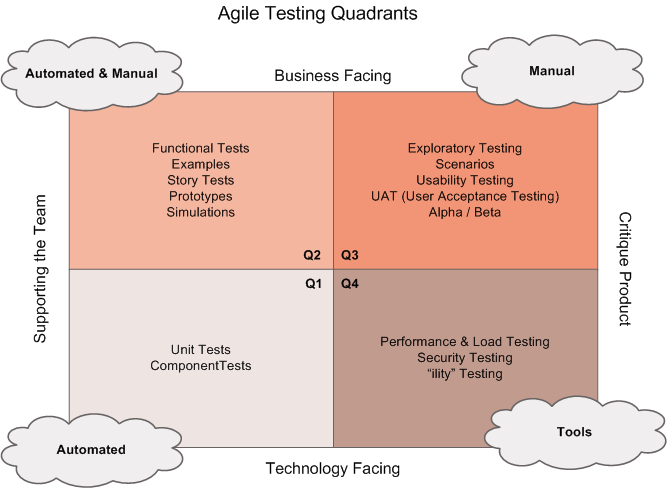
\includegraphics[width=\linewidth]{pics/agile-testing-quadrants.png}
	\caption{\textit{Agile Testing Quadrants} nach Lisa Crispin (\url{https://lisacrispin.com/2011/11/08/using-the-agile-testing-quadrants/})}
	\label{fig:agile-testing-quadrants}
\end{figure}

\subsubsection{Q1: automatisiert}

Im ersten Quadranten geht es um Tests, die vollautomatisch ausgeführt werden können. Diese Tests sollen in einer CI-Umgebung nach jedem Push und vor jedem Merge durchlaufen. Scheitert ein Test, wird der Entwickler notifiziert. Ein Merge-Request soll nicht ausgeführt werden können, wenn Testfälle im Feature-Branch scheitern, sodass die Tests im Master-Branch immer durchlaufen.

Einzelne Funktionen können durch \textit{Unit Tests} abgedeckt werden. Da die Sichtbarkeitsregeln in Go anders geregelt sind als in Java, und ein Unit Test jeweils zum gleichen Modul wie der zu testende Code gehört, können auch interne Funktionen getestet werden, und nicht nur die vom Modul exportierte Schnittstelle \cite[p. 311]{gopl}. Dies erlaubt ein feingranulareres Testing auf Stufe Unit Test.

Die Komponententests sind dann als Tests einzelner Module und somit als Black-Box-Tests zu verstehen, wobei die exportierte (d.h. öffentliche) Schnittstelle angesprochen wird. Auf Mocking soll hierbei verzichtet werden, da das Schreiben \textit{Test Doubles} (Mocks, Spies, Fakes) Kenntnisse der Implementierung und nicht nur der Schnittstelle erfordert. Ändert sich die Implementierung bei gleichbleibendem (und weiterhin erfülltem) Schnittstellenvertrag, sollte auch ein Komponententest weiterhin funktionieren. Dies ist beim Einsatz von Mocks oft nicht gegeben. Eric Elliot bezeichnet Mocking gar als ein \textit{Code Smell}, das die Struktur des Codes verkompliziere, wo doch \textit{Test Driven Development} dabei helfen solle, Code zu vereinfachen \cite[p. 205]{composingsoftware}, 

Ziel der Unit- und Komponententests ist nicht eine möglichst hohe Codeabdeckung, sondern ein optimales Verhältnis von Aufwand und Ertrag: Zeigt es sich, dass für einzelne Tests mit viel Aufwand eine umfassende Umgebung (im weitesten Sinne) aufgebaut werden muss, soll stattdessen geprüft werden, ob der Code nicht besser mittels Tests des zweiten Quadranten getestet werden soll.

\subsubsection{Q2: automatisiert und manuell}

Im zweiten Quadranten geht es um Tests auf der funktionalen Ebene, die teils automatisch, teils manuell ausgeführt werden.

Da \texttt{px} nicht nur interaktiv, sondern auch in Skripten verwendet werden soll, können komplette Workflows ebenfalls vollautomatisiert durchgetestet werden. Ein folgendes Skript könnte etwa folgenden Ablauf beschreiben:

\begin{itemize}
	\item Einloggen auf einen System mit speziellen Test-Zugangsdaten
	\item Hochladen mehrerer Dokumente inklusive Metadaten mit Abspeicherung der dabei generierten Dokument-UUIDs
	\item Tagging der hochgeladenen Dokumente
	\item Herunterladen der zuvor hochgeladenen Dokumente und Vergleich mit dem ursprünglich hochgeladenen Dokument (etwa per SHA-2-Prüfsumme)
	\item Abfragen der zuvor mitgeschickten Metadaten und Tags; Prüfung derselben gegenüber den Ausgangsdaten
\end{itemize}

Ein solcher Test muss zwangsläufig gegen eine laufendes Umgebung durchgeführt werden. (Ähnliche, aber wesentlich einfachere Abläufe werden bereits mit Uptrends durchgeführt, um die Verfügbarkeit der produktiven Umgebung automatisch zu überprüfen.) Hierbei besteht die Gefahr, dass Testfälle aufgrund eines Fehlers in der entsprechenden Umgebung scheitern, und nicht aufgrund der am Code von \texttt{px} vorgenommenen Änderungen. Im schlimmsten Fall müsste ein Merge-Vorgang auf den Master-Branch aufgrund einer nicht funktionierender Umgebung verzögert werden. Eine pragmatische Lösung wäre es, wenn diese Tests gegen die produktive Umgebung ausgeführt würden. Diese Umgebung ist hoch verfügbar, und bei den seltenen Ausfällen derselben könnte auch notfalls mit einem Merge-Vorgang auf den Master-Branch zugewartet werden.\footnote{Der Autor dieser Zeilen ist u.a. auch für die Verfügbarkeit des Produktivsystems zuständig. Ist diese nicht gegeben, werden Entwicklungsarbeiten erfahrungsgemäss unterbrochen, bis das System wieder vollumfänglich verfügbar ist.} Die Zugangsdaten für ein entsprechendes Testkonto können innerhalb der CI-Umgebung als verschlüsselte Variablen und lokal als Umgebungsvariablen abgelegt werden.

Das Schreiben von Skripts ist meistens ein Prozess, dem üblicherweise mehrere manuelle Durchgänge der auszuführenden Arbeitsschritte vorangeht. Skripts werden häufig dann geschrieben, wenn ein manueller Vorgang die Finger stärker beansprucht als den Kopf, und aufgrund der nachgebenden Achtsamkeit die Gefahr für Flüchtigkeitsfehler besteht. So soll es auch im vorliegenden Projekt gehandhabt werden: Wird ein neues Feature eingebaut, d.h. eine neue \textit{User Story} umgesetzt, und sich das Testing desselben als aufwändig herausstellt, soll ein Testskript geschrieben werden, das dann sogleich in die CI-Pipeline eingebaut werden kann. Manuelle Tests sollen so möglichst bald und unkompliziert in automatisierte überführt werden.

\subsubsection{Q3: manuell}

Nach jedem Sprint erhalten die Entwickler bei PEAX Zugang zum aktuellen Stand der Software mit einem Changelog. Sie haben nun eine Woche Zeit, sich mit den neuen Features vertraut zu machen, und auszuprobieren, ob sich die Software wie gewünscht verhält.

Hier geht es weniger um die Korrektheit gemäss Spezifikation (Akzeptanzkriterien in den User Stories), welche bereits durch Tests in Q1 und Q2 gewährleistet werden sollte, sondern um \textit{User Acceptance Tests}. Hiermit wird geprüft, ob das Inkrement die Bedürfnisse der Benutzer erfüllt und ihren Zielen dient. «Another kind of acceptance testing is \textit{user acceptance testing}. Commonly used in Agile environments, user acceptance testing (UAT) checks that the system meets the goals of the users and operates in a manner acceptable to them \cite[p. 85]{testing}.

Auch soll im Rahmen dieser Tests die \textit{Usability} des Inkrements überprüft werden. Stossen mehrere Tester auf die gleichen Probleme? Wurde ein Feature (z.B. ein Subcommand) schlecht benannt, sodass dessen Semantik unklar ist? Ist die angebotene Hilfe-Funktion zu einem Befehl unklar oder schlecht formuliert?

Die Tests in Q3 sind jeweils in der ersten Wochenhälfte nach einem Sprint durchzuführen, sodass die Rückmeldungen für die Planung des nächsten Sprints, der in der darauffolgenden Woche startet, berücksichtigt werden kann.

\subsubsection{Q4: Tools}

Für die Qualitätssicherung können verschiedene Werkzeuge zum Einsatz kommen:

\begin{description}
	\item[Benchmarks]: Bieten sich bei der Implementierung einer performancekritischen Funktion mehrere Varianten an, ist die bessere Variante mithilfe von Benchmarks zu bestimmen. Die integrierte Benchmark-Funktion des \texttt{go}-Tools\footnote{\texttt{go test -bench=[pattern]}}, die eine Funktion so oft laufen lässt, bis eine statistisch relevante Aussage über deren Performance gemacht werden kann, ist hierzu völlig ausreichend \cite[p. 321]{gopl}.
	\item[Profiling]: Im Profiling geht es darum, die kritischen Stellen im Code im Bezug auf Rechenzeit, Speicherverbrauch und blockierende Operationen zu ermitteln, um Aufgrund dieser Erkenntnis effektive Optimierungen am Code vornehmen zu können (Flaschenhalsoptimierung). Hierzu bietet das \texttt{go}-Tool\footnote{\texttt{go test -cpuprofile/-memprofile/-blockprofile=[Ausgabedatei]}} wiederum sehr mächtige Werkzeuge out-of-the-box an \cite[p. 324]{gopl}.
	\item[Quellcodeanalyse]: Kompilierbarer und korrekter Quellcode ist nicht automatisch auch guter Quellcode im Bezug auf Klarheit, Einfachheit, Eleganz und Best Practices. Beispielsweise sollen nach Möglichkeit keine veralteten und unsicheren APIs verwendet werden. Exportierte Funktionen, d.h. die öffentliche Schnittstelle eines Moduls, muss dokumentiert sein. Hierzu gibt es einerseits das Tool \texttt{go vet}\footnote{Vet examines Go source code and reports suspicious constructs, such as
		Printf calls whose arguments do not align with the format string.}, das zum Lieferumfang von Go gehört, und potenzielle Fehler im Code meldet. Das Zusatztool \texttt{golint}\footnote{\url{https://github.com/golang/lint}} meldet stilistische Unschönheiten im Code.
\end{description}

Da es bei diesen Tools nicht um kategorische Qualitätskriterien (richtig oder falsch), sondern eher um kontinuierliche (schnell/langsam, hoher/tiefer Speicherverbrauch, hohe/tiefer Quellcodequalität) handelt, die einer subjektiven Interpretation bedürfen, sollen diese Tools nicht Teil der CI-Pipeline sein, sondern kontinuierlich (\texttt{go vet} und \texttt{golint}) und bei konkretem Bedarf (Benchmarking, Profiling) im Entwicklungsprozess eingesetzt werden. Um eine gewisse Quellcodeanalyse gewährleisten zu können, ist die Ausgabe von \texttt{go vet} und \texttt{golint} am Ende eines jeden Sprints summarisch zu dokumentieren.\footnote{Da die Ausformulierung von Rechtfertigungen oftmals anstrengender ist als die notwendigen Korrekturen am Code vorzunehmen, ist diese Massnahme als Anreiz zu verstehen, die erhaltenen Warnungen zu behandeln statt zu ignorieren.}

\newpage

\section{Realisierung}
\label{sec:Realisierung}

Wie im Anhang (\secref{sec:Entscheidung-Programmiersprache}) beschrieben und begründet, wird \texttt{px} mit \textsc{Go} umgesetzt. Da die Standard Library von \textsc{Go} sehr umfassend ist, die mit dem Package \texttt{net/http} über einen mächtigen HTTP-Client (und Server) verfügt, wird nur eine Fremdkomponente (Zugriff auf den Keystore) eingesetzt.

Enorm hilfreich in der Umsetzung war Standardwerk zu \textsc{Go} \cite{gopl}, das nicht nur die Programmiersprache beschreibt, sondern auch deren idiomatischen Gebrauch.

\subsection{Architektur: Package-Übersicht}

\textsc{Go}-Code wird in sogenannte Packages aufgeteilt. Da das Projekt in \textsc{GitLab} \texttt{px} heisst, wird das Hauptpackage als \texttt{px} benannt. Im Root-Verzeichnis befindet sich kein \textsc{Go}-Code.\footnote{\texttt{px.go} beinhaltet bloss eine Package-Deklaration mit einem entsprechenden Kommentar.} Dieser ist in verschiedenen Unterverzeichnissen (\texttt{requests}, \texttt{tokenstore}, usw.) abgelegt. Die Dateien in den Unterpackages deklarieren ihre Packagezugehörigkeit jeweils mit dem unmittelbaren Überverzeichnis, also beispielsweise nicht \texttt{px/tokenstore}, sondern nur \texttt{tokenstore}. Bei der Verwendung der Packages hingegen wird der ganze Pfad angegeben: \texttt{px/tokenstore}.

Der Code für das ausführbare Programm (\texttt{px.go}) befindet sich gemäss Konvention\footnote{\url{https://github.com/golang-standards/project-layout\#cmd}} im \texttt{cmd}-Unterverzeichnis \cite[S. 12]{powerful-cli-apps-in-go}. Das Package heisst jedoch nicht \texttt{cmd}, sondern \texttt{main}, und verfügt über eine Funktion namens \texttt{main} als Haupteinstiegspunkt. Somit ist \texttt{px} als Library, und \texttt{cmd/px.go} als Client dieser Library zu verstehen.\footnote{Da sich nur knapp ein Viertel des Programmcodes im Client-Teil befinden, könnte auf Basis der \texttt{px}-Library recht einfach ein alternativer Client umgesetzt werden.} Die Projektstruktur ist auf der linken Seite der \imgref{img:Komponentendiagramm} zu sehen. Die einzelnen Packages haben folgende Verantwortlichkeiten:

\begin{figure}
    \centering
    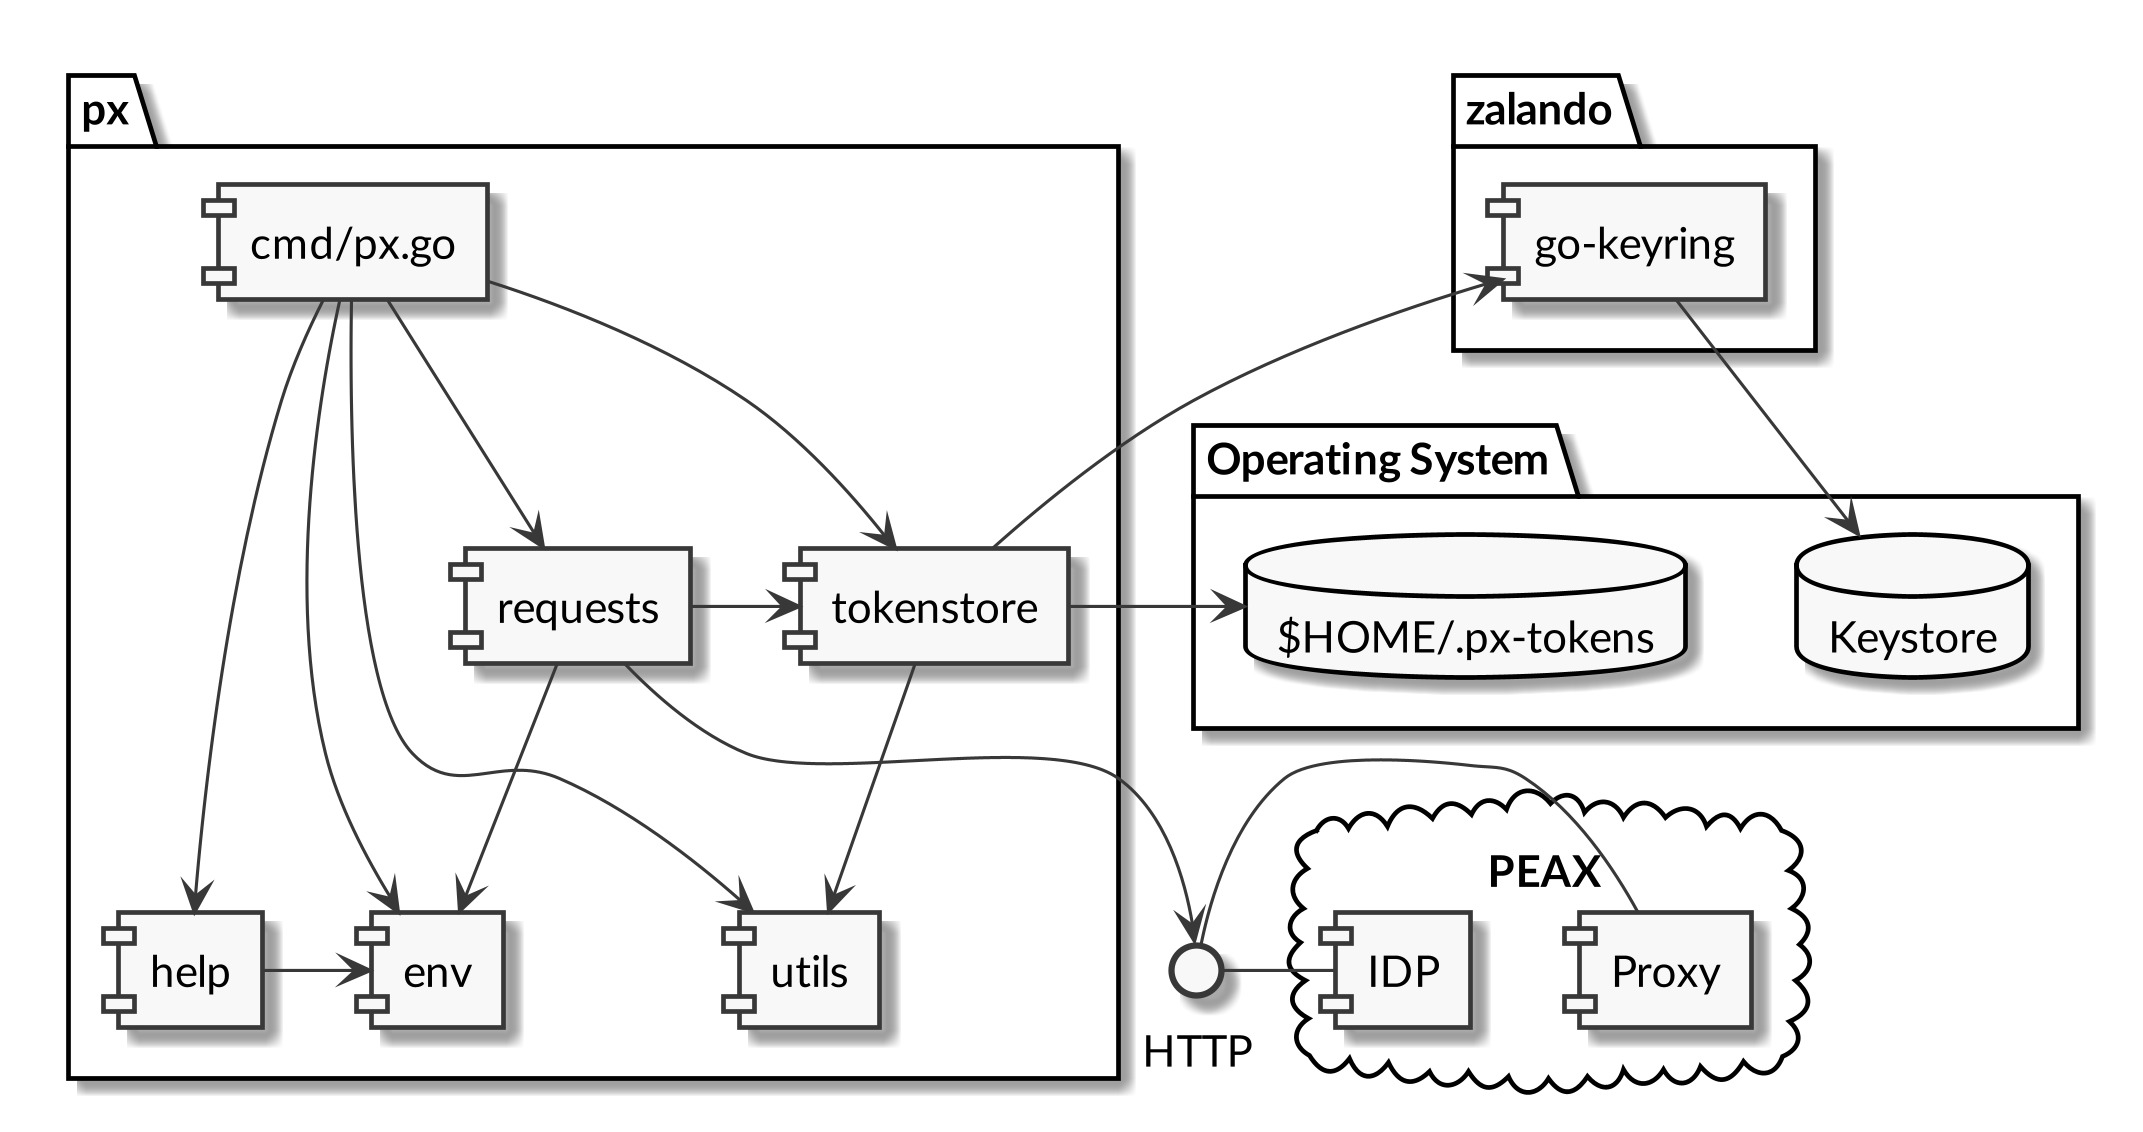
\includegraphics[width=\linewidth]{pics/komponentendiagramm.png}
    \caption{Die Package-Struktur von \texttt{px} (Komponentendiagramm)}
    \label{img:Komponentendiagramm}
\end{figure}

\begin{description}
    \item[\texttt{env}] Die Umgebungen (\secref{sec:Umgebungen}) sind in diesem Package aufgelistet. Jede Umgebung verfügt über ein URL-Schema, womit (via Proxy) auf das Backend und direkt auf den IDP zugegriffen werden kann. Verschiedene Funktionen bieten die Möglichkeit, URLs für den Ressourcenzugriff anhand der jeweiligen Umgebung und weiterer Parameter zu erzeugen, was mit dem Unit Test \texttt{env\_test.go} überprüft wird. Die Standardeinstellung, welcher Keystore (sicher/unsicher) zu verwenden ist, wird statisch pro Umgebung definiert.
    \item[\texttt{help}] Dieses Package umfasst die Hilfetexte. Zu jedem Befehl gibt es jeweils eine kurze, einzeilige Beschreibung, und einen ausführlichen Hilfetext. Dieses Package importiert das \texttt{env}-Package, damit bei der Hilfe zum Login-Befehl (\texttt{px login}) die verfügbaren Umgebungen automatisch aufgelistet werden können.
    \item[\texttt{tokenstore}] Hier sind zentrale Datenstrukturen für das Token-Handling mit dazugehörigen Funktionen definiert. Die Datenstruktur \texttt{TokenPair} dient zur lokalen, persistenten Speicherung von Tokens. Sie wird auf Basis einer \texttt{TokenResponse} aufgebaut, indem Informationen extrahiert und anhand von Kontextinformationen ergänzt. Die Datenstruktur \texttt{TokenStore} speichert pro Umgebung und Token-Typ (\texttt{agent}, \texttt{user}) ein \texttt{TokenPair} ab. Der \texttt{TokenStore} wird als JSON-Struktur serialisiert und im \texttt{\$HOME}-Verzeichnis des Benutzers abgespeichert. Der Zugriff auf den sicheren Keystore ist ebenfalls hier implementiert.
    \item[\texttt{requests}] In diesem Package sind die eigentlichen Zugriffe auf die API via HTTP umgesetzt. Hier sind Datenstrukturen für die Credential-Payloads mit dazugehörigen Funktionen definiert, die für Login-Vorgänge verwendet werden (\texttt{credentials.go}. Für die verschiedenen Befehle (\texttt{login}, \texttt{get}, \texttt{upload} usw.) sind hier dazugehörige Funktionen definiert. Der transparente Retry-Mechanismus ist ebenfalls hier implementiert (\texttt{requests.go}). Das Package \texttt{tokenstore} wird verwendet, um die Requests mit den notwendigen Authentifizierungsinformationen (\texttt{Authentication}-Header) auszustatten.
    \item[\texttt{utils}] Dieses Package umfasst verschiedene Funktionen, die von verschiedenen anderen Packages und vom Hauptprogramm verwendet werden, jedoch nicht direkt zu den jeweiligen anderen Packages gehören. Die Eingabeaufforderung für Passwörter (sicher über ein SSH-Terminal, d.h. ohne Echo) ist etwa hier umgesetzt (\texttt{pwinput.go} und \texttt{pwinput\_windows.go}\footnote{Aufgrund eines offenen Fehlers (\url{https://github.com/golang/go/issues/34461}) funktioniert die sichere Passworteingabe nicht unter \textsc{Windows}. Aus diesem Grund wird mithilfe eines Build Constraints (\url{https://golang.org/pkg/go/build/\#hdr-Build\_Constraints}) für den \textsc{Windows}-Build eine unsichere Variante, für alle anderen Betriebssysteme die sichere Variante verwendet.}). Weiter gibt es Funktionen zum automatischen Ermitteln des MIME-Types einer Datei, und eine Funktion zur rekursiven Auflisten lesbarer Dateien in einem Unterverzeichnis.
    \item[\texttt{cmd/px.go}] Dies ist der eigentliche Command Line Client mit der Einstiegsfunktion \texttt{main}. Die zur Verfügung stehenden Befehle weden in einer Map namens \texttt{commands} abgespeichert, wobei der Befehlsname den Key bildet, und der Wert eine Datenstruktur bestehend aus einer Funktionsreferenz, dem einzeiligen Infotext und dem längeren Hilfetext (siehe Package \texttt{help}) zusammengesetzt ist. Die \texttt{main}-funktion prüft, ob der eingegebene Befehl in der Map gefunden wurde, und führt diese dann aus. Jede dieser Command-Funktionen nimmt den \texttt{TokenStore} als Argument entgegen, und gibt einen optionalen Fehler zurück.\footnote{Die Befehle \texttt{help} und \texttt{env} bilden eine Ausnahme.} Der \texttt{TokenStore} wird zu Beginn von \texttt{main} aus \texttt{~/.px-tokens} geladen, und am Ende (mit möglichen Änderungen) wieder in diese Datei zurückgeschrieben.\footnote{Die sicher verwahrten Tokens werden bei Bedarf, d.h. bei einem entsprechenden Request, nachgeladen.} Die einzelnen Command-Funktionen sind selber für ihre Seiteneffekte (Ausgabe möglicher Payloads) verantwortlich. Die Fehlerausgabe wird über die Rückgabe eines Fehlers in \texttt{main} abgehandelt. Die Flags sind ebenfalls für jeden Befehl eigens definiert, wobei Gemeinsamkeiten in Hilfsfunktionen und Konstanten (Beschreibungstexte) ausgelagert sind. Das Parsen der Kommandozeilenargumente wird vom sehr mächtigen und komfortablen \texttt{flag}-Package übernommen, das Teil der Standard Library von \textsc{Go} ist. Tritt bei der Programmausführung ein Fehler auf, wird einerseits eine Fehlermeldung auf \texttt{stderr} geschrieben, andererseits der Rückgabewert \texttt{1} an den aufrufenden Prozess zurückgegeben.\footnote{Im Gegensatz zu \texttt{0}, das für eine erfolgreiche Ausführung steht.} Dieser Rückgabecode wird in den Testskripts über die Shell-Variable \texttt{\$?} geprüft.
\end{description}

\subsection{Zwei-Faktor-Authentifizierung}

Hat ein Benutzer im Portal die Zwei-Faktor-Authentifizierung über SMS oder TOTP aktiviert, wird der initiale Login-Request mit Benutzername und Passwort mit dem HTTP-Status 380 quittiert. Diese Antwort enthält auch die Information, welcher zweite Faktor (SMS oder TOTP) verlangt wird.

Dem Benutzer wird eine entsprechende Eingebeaufforderung angezeigt. Nach der Eingabe wird der initiale Request mit dem eingegebenen zweiten Faktor ergänzt und erneut an den IDP gesendet. Hat der Vorgang funktioniert, erhält der Benutzer das Token-Pair, das im Keystore für die spätere Verwendung abgelegt wird.

Dieser Vorgang ist in \imgref{fig:2fa} mit einem Sequenzdiagramm veranschaulicht.

\begin{figure}
    \centering
    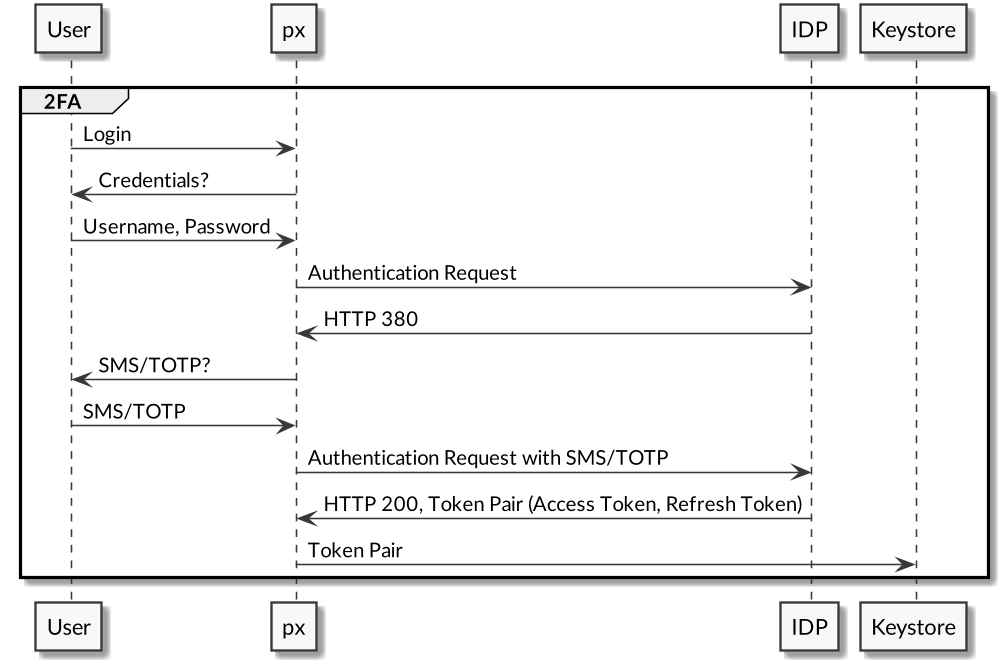
\includegraphics[width=\linewidth]{pics/sequence-2fa.png}
    \caption{Der Ablauf der Zwei-Faktor-Authentifizierung mit SMS oder OTP (Sequenzdiagramm)}
    \label{fig:2fa}
\end{figure}

\subsection{Token Store}
\label{sec:Realisierung-Token-Store}

Für jede Umgebung ist mit dem Flag \texttt{Confidential} definiert, ob die Tokens standardmässig sicher oder unsicher verwahrt werden sollen. Wie im Abschnitt \secref{sec:Konzept-Token-Store} beschrieben kann diese Einstellung mit den entsprechenden Flags übersteuert werden.

Wurde die unsichere Variante gewählt bzw. beibehalten, werden die beiden Tokens direkt in die JSON-Struktur geschrieben, die vor Beendigung des Clients nach \texttt{~/.px-tokens} geschrieben wird. Für jede Kombination von Token-Art (\texttt{user} oder \texttt{agent}) und Umgebung (\texttt{test}, \texttt{stage} usw.) wird je ein Feld \texttt{refresh\_token} und \texttt{access\_token} gespeichert. Als zusätzliches Feld wird \texttt{use\_keystore} mit dem Wert \texttt{false} abgespeichert.

Wird jedoch die sichere Variante gewählt bzw. beibehalten, wird unter der Kombination von Token-Art und Umgebung kein Token Pair abgespeichert, sondern bloss das Feld \texttt{use\_keystore} mit dem Wert \texttt{true}, was bei künftigen Token-Zugriffen als Verweis auf den nativen Keystore zu verstehen ist.

Das folgende Codebeispiel zeigt einen verkürzten Auszug aus der Datei \texttt{~/.px-tokens}, wobei für die Umgebung \texttt{test} die unsichere und für die Umgebung \texttt{stage} die sichere Token-Verwahrung verwendet worden ist.

\begin{lstlisting}[caption={Die JSON-Struktur für den Keystore (Auszug)}]
{
	"tokens": {
		"user_test": {
			"access_token": "eyJhbGciOiJSUz...",
			"refresh_token": "eyJhbGciOiJIUz...",
			"use_keystore": false
		},
		"user_stage": {
			"use_keystore": true
		}
	},
	"default_environment": "stage"
}
\end{lstlisting}

Der sichere Keystore ist als Key-Value-Store mit globalem Namensraum zu verstehen. Die Keys müssen also vollständig qualifiziert sein, d.h. alle Informationen enthalten, die etwa einen Refresh Token von \texttt{px} für einen Benutzer auf der Umgebung \texttt{prod} von einem auf dem Computer hinterlegten E-Mail-Passwort oder dergleichen unterscheidet. Hierzu wurde das folgende Namensschema (Zeile 1) gewählt:

\begin{lstlisting}[caption={Namensschema für die Keys auf dem nativen Keystore (mit Beispielen)},numbers=left]
px:[environment]:[(user|agent)]:[(refresh|access)Token]
px:test:user:refreshToken
px:prod:agent:accessToken
\end{lstlisting}

Zeile 2 zeigt den Key für einen Refresh Token für die User API auf der Umgebung \texttt{test}. Auf Zeile 3 ist ein Key für einen Access Token für die Agent API auf der Umgebng \texttt{prod} zu sehen.

\subsubsection{Fremdkomponente \texttt{zalando/go-keyring}}
\label{sec:Go-Keyring}

Da sich der Zugriff auf den sicheren Keystore von Plattform zu Plattform unterscheidet, wurde dieser Mechanismus nicht selber implementiert. Das Package \texttt{go-keyring} von \textsc{Zalando}\footnote{\url{https://github.com/zalando/go-keyring}} löst dieses Problem bereits ‒ und funktionierte auf Anhieb.

Das Package \texttt{go-keyring} wird nur im Package \texttt{tokenstore} verwendet, und sonst nirgends in \texttt{px}. Mithilfe der Funktionen \texttt{keyring.Set}, \texttt{keyring.Get} und \texttt{keyring.Delete} kann Secret abgespeichert, gelesen und gelöscht werden. Zu jedem Key wird nicht nur ein Passwort (das eigentliche Secret), sondern auch ein Benutzername abgelegt. Als Passwort dient jeweils der Token. Als Benutzername wurde der Vollständigkeit halber der String \texttt{"px"} verwendet.\footnote{Für \texttt{px} spielt es keine Rolle, \textit{welcher} Benutzer eingeloggt ist. Validierungen auf den Scope zur Verhinderung von Fremdzugriffen werden serverseitig geprüft. Der Benutzer von \texttt{px} soll auch solche Zugriffe versuchen können, ohne schon clientseitig abgeblockt zu werden, um etwa Angriffe simulieren zu können.}

Diese drei Funktionen werden durch die eigenen Funktionen \texttt{storeSecret}, \texttt{loadSecret} und \texttt{deleteSecret} (\texttt{tokenstore/tokenpair.go}) gewrappt, wobei zusätzlich ein einheitliches Key-Format über die Funktion \texttt{tokenKeys} sichergestellt wird.

\subsection{Retry-Mechanismus}
\label{sec:Retry-Mechanismus}

Im Konzept (\secref{sec:Token-Refresh}) wurde beschrieben, nach welcher Strategie die Tokens aktualisiert werden sollen. Das Sequenzdiagramm \imgref{fig:retry-mechanism} zeigt, wie dies umgesetzt worden ist.

\begin{figure}
    \centering
    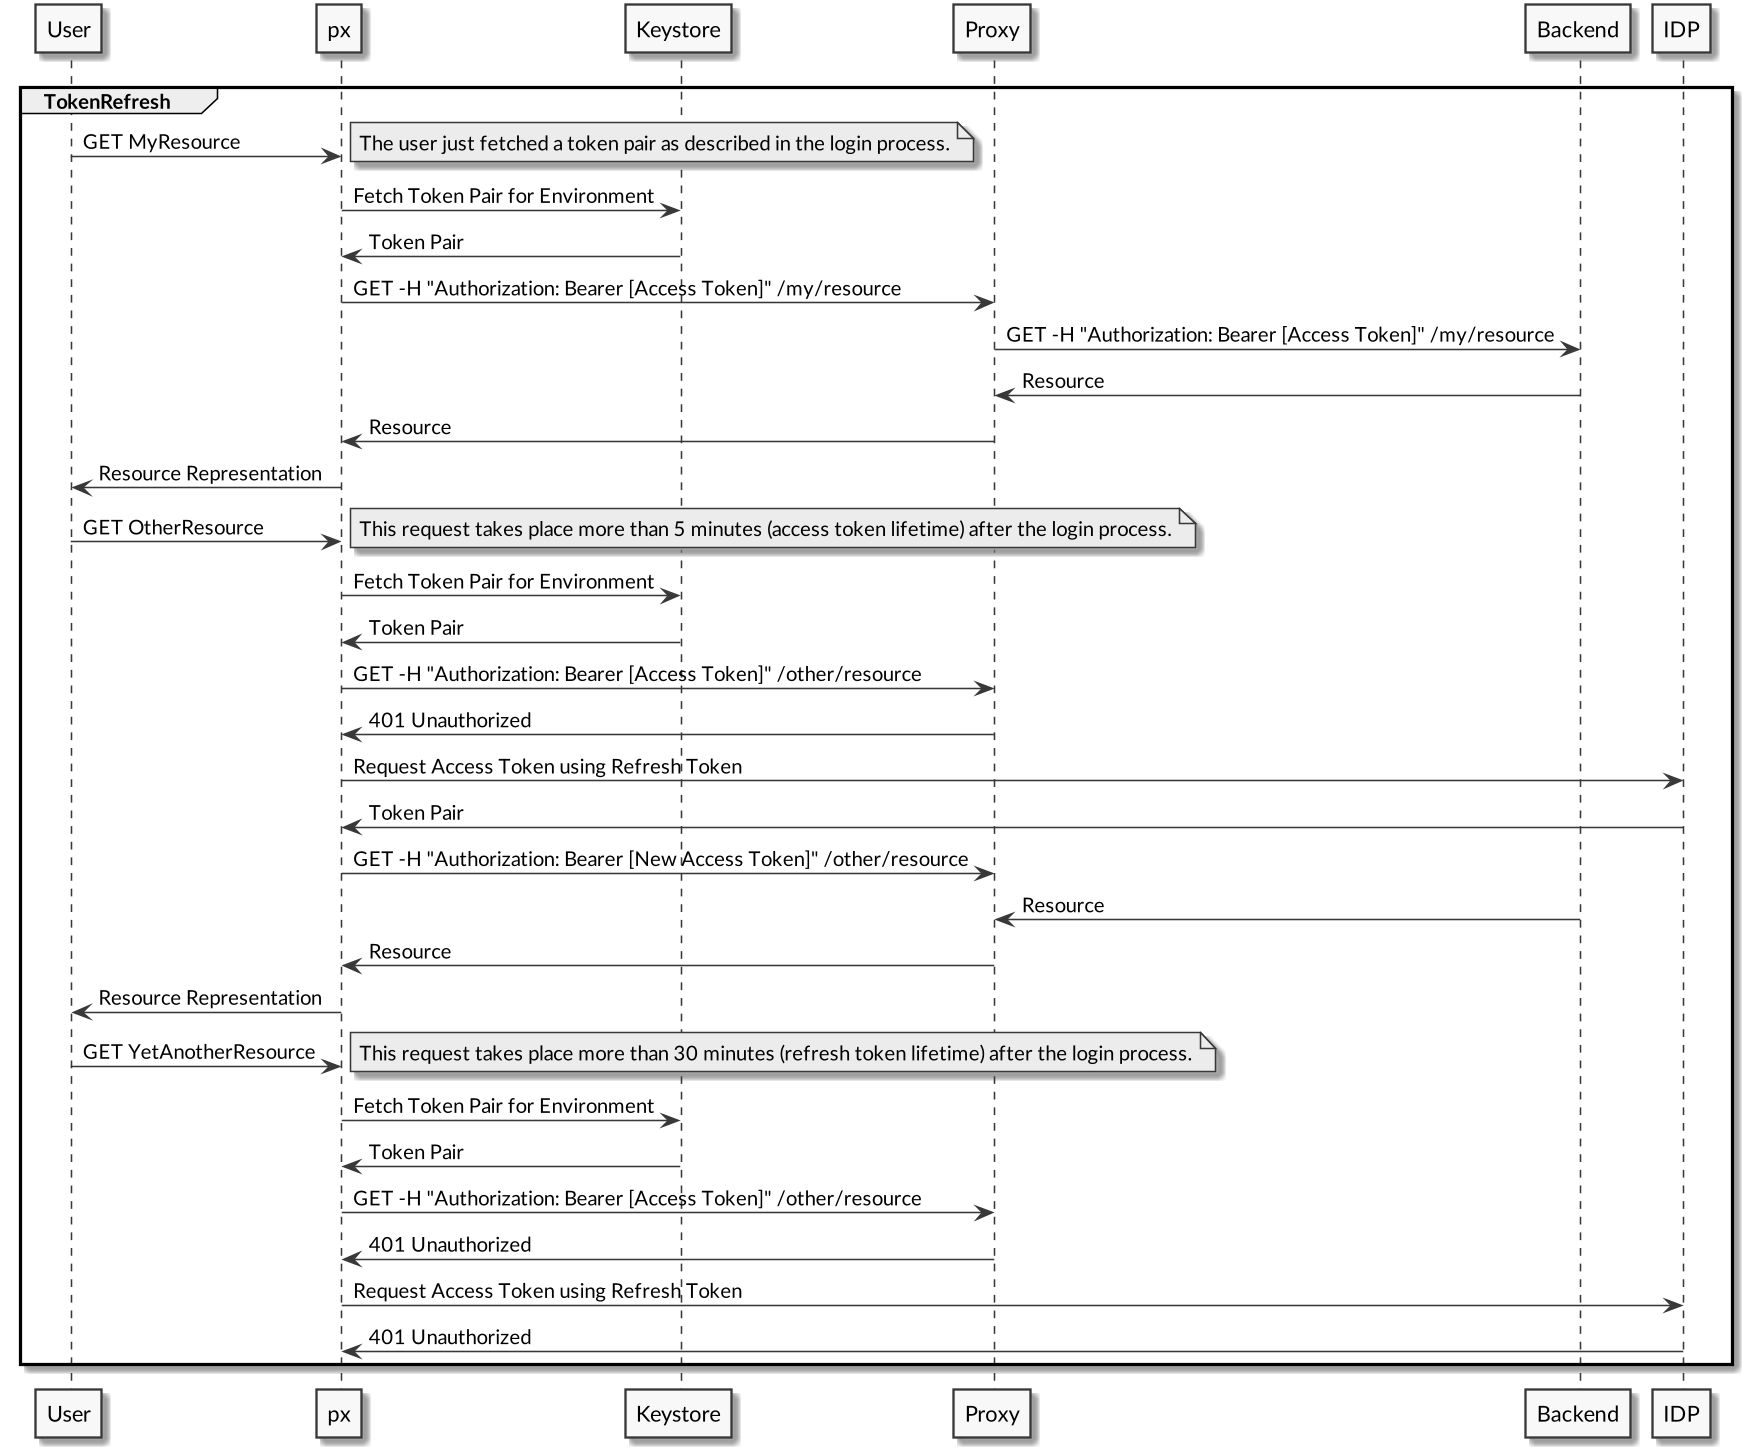
\includegraphics[width=\linewidth]{pics/sequence-retry.png}
    \caption{Der für den Benutzer transparente Retry-Mechanismus mit einem Token Pair, das im Hintergrund automatisch aktualisiert wird (Sequenzdiagramm)}
    \label{fig:retry-mechanism}
\end{figure}

Einige Implementierungsdetails, die auf dem Sequenzdiagramm nicht ersichtlich sind, sollen an dieser Stelle noch erläutert werden.

Der erste, naive Implementierungsversuch, der darin bestand, einen gescheiterten Request (mit HTTP-Status \texttt{401 Unauthorized}) mit aktualisiertem \texttt{Authorization}-Header einfach erneut abzuschicken, scheiterte für Requests, die über einen Body verfügen, was bei \texttt{POST}, \texttt{PUT} und \texttt{PATCH} der Fall ist. Grund dafür ist, dass die Repräsentation des Bodies bei einem ausgeführten Request konsumiert wird, und anschliessend nicht mehr verwendet werden darf.

Technisch war dies zunächst so implementiert worden, dass die Funktion \texttt{doWithToken\-Refresh} (\texttt{requests/requests.go}) als Parameter (nebst Kontextinformationen zum Auffinden der richtigen Tokens) einen Request erwartete. Die einzelnen Request-Funktionen (\texttt{Get}, \texttt{Post}, \texttt{Put}, \texttt{Patch} usw.) erstellten den initialen Request und übergaben ihn an \texttt{doWith\-Token\-Refresh}, welches dann anhand des Token Stores einen Token Refresh durchführte, und den initialen Request mit aktualisiertem \texttt{Authorization}-Header erneut abschickte.

Die Lösung für das Problem mit den konsumierten Bodies konnte gelöst werden, indem für jeden erneuten Versuch ein neuer Request aufgebaut wird. Da \texttt{doWithTokenRefresh} jedoch nicht über alle Informationen verfügen kann, welche zum Erstellen eines Requests nötig sind, musste ein Weg gefunden werden, diese Kontextinformationen für alle möglichen Arten von Requests mitliefern zu können. Da \textsc{Go} \textit{first class functions} unterstützt, konnte dies sehr elegant mit einer Closure gelöst werden \cite[S. 136]{gopl}. Die Client-Funktion übergibt nicht mehr einen Request, sondern eine Funktion, die einen Request erstellt. Die Kontextinformationen zur Erstellung des Requests erhält sie von der umschliessenden (\textit{enclosing}) Funktion; den aktualisierten Access Token erhält sie zu einem späteren Zeitpunkt als Parameter, nachdem \texttt{doWithTokenRefresh} das Token Pair aktualisiert hat.\footnote{Wäre \texttt{px} mit einer stark objektorientierten Programmiersprache wie \textsc{Java} oder \textsc{C++} umgesetzt worden, dürfte an dieser Stelle wohl ein Klassendiagramm mit \texttt{AbstractRequestFactory}, \texttt{GetRequestFactoryImpl} und dergleichen stehen. \textsc{Peter Norvig} hat demonstriert, dass in funktionalen Programiersprachen 16 der 23 \textsc{GoF}-Patterns \textit{«invisible or simpler»} sind (\url{http://www.norvig.com/design-patterns/design-patterns.pdf}). Die Implementierung von \texttt{doWithTokenRefresh} veranschaulicht dieses Prinzip.}

\subsection{Umgang mit Risiken}

Von den ermittelten Risiken (\secref{sec:Risikoanalyse} sind bei der Umsetzung v.a. die technischen und sicherheitsrelevanten Risiken relevant. Mit ihnen wurde folgendermassen verfahren:

\begin{description}
    \item[Token-Verwahrung] Mit dem nativen Keystore wurde eine Lösung gefunden, die so sicher ist, wie der Keystore des zugrundeliegenden Betriebssystems. Möchte der Benutzer von \texttt{px} die Tokens der Produktivumgebung im Klartext abspeichern, muss er das explizit angeben. Die Kombination aus sicheren Grundeinstellungen und der Möglichkeit, diese bei Bedarf zu übersteuern, hat der Anwender eine standardmässig sichere, jedoch ausreichend flexible Lösung.
    \item[Payment-Schnittstelle] Hat der Benutzer ein Bankkonto hinterlegt, und loggt er sich mit \texttt{px} auf das Produktivsystem ein, kann er Zahlungen mit den entsprechenden Requests in Auftrag geben. Es bestehen die gleichen Risiken wie bei der Bedienung des Portals. Auf eine unnötige und willkürliche Einschränkung der API-Abdeckung wurde verzichtet. Das Risiko liegt ganz beim Benutzer; die Sicherheit steht und fällt mit der Token-Verwahrung, welche sicher genug umgesetzt worden ist.
\end{description}

\subsection{Notizen zur Implementierung und zum Testing}

Während der Umsetzung von \texttt{px} wurden zu jeder User Story Umsetzungsnotizen und Testprotokolle geschrieben, die im Zusatzdokument \textit{Backlog} (\secref{apx:WeitereDokumente}) zu finden sind. Da dieses Dokument recht umfassend ist, ist es als Referenz zu lesen. Hierbei ist jedoch zu beachten, dass das Dokument, gerade die Auflistung der User Stories, historisch gewachsen ist: Notizen früherer Stories wurden teils durch Notizen späterer Stories obsolet gemacht. Es empfiehlt sich also, bei der Lektüre so weit unten wie möglich ‒ d.h. bei der jeweiligen Story, die von Interesse ist ‒ einzusteigen, und bei Unklarheiten weiter oben nachzulesen, um den Hintergrund besser erfassen zu können.

Aufgrund der agilen Vorgehensweise gibt es keine umfassenden Testpläne und Testprotokolle, zumal das Testen nicht als von der Implementierung getrennte Phase praktiziert worden ist. Eine Ausnahme bilden die wenigen manuellen Tests (Regressionstests), die ab Sprint 3 jeweils durchgeführt worden und am Ende des \textit{Backlog}-Dokuments verzeichnet sind.

\newpage

\section{Evaluation und Validierung}

Das vorliegende Projekt entstammt dem PEAX-Ideation-Prozess, worin sich Entwicklungs- und Validierungsphase abwechseln. 

\subsection{Rückmeldungen von Entwicklern}

Nach jedem Sprint wird ein Inkrement an die Entwickler ausgeliefert (siehe \secref{sec:Vorgehen}). Die Rückmeldungen werden hier gesammelt und kommentiert ‒ und fliessen in den jeweils nachfolgenden Sprint ein.

\subsubsection{Sprint 1}

\begin{itemize}
    \item \textsc{Michael Buholzer} wünscht sich Erfolgs- und Vollzugsmeldungen nach dem Login oder dem Upload eines Dokuments.
    \begin{itemize}
        \item \texttt{stdout} sollte grundsätzlich «sauber» bleiben, d.h. frei von unnötigen Ausgaben, die ein nachgelagertes Programm wieder herausfiltern müsste. Eine wichtige Maxime von UNIX-Programmen lautet: \textit{«Expect the output of every program to become the input to another, as yet unknown, program.»} \cite[p. 3]{unixtimesharing}. Siehe dazu auch \textit{Rule of Silence} \cite[p. 20]{unixart} und \textit{Silence is Golden} \cite[p. 111]{unixphil}.\footnote{Brian W. Kernighan berichtet von der Zeit, als die Pipe Einzug in UNIX hielt, womit die Ausgabe eines Programms zur Eingabe eines anderen Programms gemacht werden konnte: \textit{«Ken [Thompson] and Dennis [Ritchie] upgraded every command on the system in a single night. […] Overall, the job was not hard—most programs required nothing more than eliminating extraneous messages that would have \textbf{cluttered a pipeline}, and sending error reports to stderr.»} \cite[p. 69]{unix-history-memoir}}
        \item \texttt{stderr} wird nicht nur als Ausgabekanal für Fehlermeldungen verwendet, sondern für Meldungen allgemein. Für Vollzugsmeldungen wäre \texttt{stderr} vorzuziehen.
        \item Da \texttt{stderr} in \texttt{px} bisher grundsätzlich für Fehlermeldungen verwendet wird, sollen Erfolgsmeldungen über ein zusätzliches Flag \texttt{-verbose}/\texttt{-v} aktiviert werden müssen.
        \item Bei anderen Anwendungsfällen signalisiert die Ausgabe des Payloads auf \texttt{stdout} den Erfolg der Operation. Beim Dokument-Upload besteht dieser beispielsweise aus der generierten UUID des hochgeladenen Dokuments.
    \end{itemize}
\item \textsc{Patrick Roos} sieht die Möglichkeit, \texttt{px} auch zur Handhabung der \textit{Vault Secrets}\footnote{\url{https://docs.ansible.com/ansible/latest/user_guide/vault.html}} (Verschlüsselung und Entschlüsselung von Benutzernamen, Passwörtern etc. zu verwenden.
    \begin{itemize}
        \item Im Arbeitsalltag von PEAX stellt die Handhabung von Vault Secrets tatsächlich eine teils mühsame und langwierige Aufgabe dar. Hier besteht durchaus Automatisierungsbedarf.
        \item \texttt{px} ist als «skriptbare» Anwendung für die PEAX API konzipiert und so potenziell für jeden PEAX-Anwender einsetzbar.
        \item Die Verwaltung und Verwendung von Vault Secrets ist hingegen eine Aufgabe im DevOps-Bereich und betrifft nur interne Entwickler bei PEAX.
        \item Eine der obersten Maximen von UNIX lautet: \textit{«Make each program do one thing well. To do a new job, build afresh rather than complicate old programs by adding new ‹features.›} \cite[p. 3]{unixtimesharing} Die Verwaltung von Vault Secrets und das Ansprechen der PEAX API sind klar zwei verschiedene Sachen und somit nicht «one thing». Die genannte Idee muss also anderweitig weiterverfolgt werden.
    \end{itemize}
\end{itemize}

\begin{itemize}
    \item \textsc{Stefano Pellegrini} fände einen Befehl \texttt{px version} sinnvoll, der die aktuelle Versionsnummer ausgibt. Damit könne man sicherstellen, dass man nicht etwa eine veraltete Version verwendet und (hinfällige) Rückmeldungen auf diese gibt.
        \begin{itemize}
            \item Tatsächlich stellen die meisten Kommandozeilentools eine solche Möglichkeit zur Verfügung, wie z.B. \textsc{Go} oder \textsc{Docker} mit den Befehlen \texttt{go version} und \texttt{docker version}. Andere Werkzeuge, wie etwa der Command Line Client von \textsc{Heroku} oder das Tool \textsc{Ripgrep} stellen ein entsprechendes Flag zur Verfügung (\texttt{heroku -v} bzw. \texttt{rg --version}).
            \item Ein Versionstag ist bereits über das Git-Repository verfügbar. Die jeweils aktuelle Version kann mittels \texttt{git describe --tags} abgerufen werden.
            \item Der Linker von \textsc{Go}\footnote{\url{https://golang.org/cmd/link/}} erlaubt es mit dem Parameter \texttt{-ldflags} uninitialisierte Strings im Programmcode mit einem Wert zu belegen.
            \item Heisst die Variable im \texttt{main}-Modul \texttt{Version}, kann die aktuelle Versionsnummer folgendermassen in die Binärdatei hineinkompiliert werden: \texttt{go build -ldflags="{}-X main.Version=\$(git describe --tags)"{} cmd/px.go}
        \end{itemize} 
    \item Weiter hat \textsc{Stefano Pellegrini} vorgeschlagen, dass \texttt{logout} sich auf die jeweils aktuelle Standardumgebung beziehen soll, damit man nicht immer eine Umgebung mit dem \texttt{-env}-Parameter angeben muss.
    \begin{itemize}
        \item Der Vorschlag ist sinnvoll und soll entsprechend umgesetzt werden.
    \end{itemize}
\item \textsc{Michael Buholzer} wünscht sich, dass die Ausgabe von JSON-Datenstrukturen automatisch formatiert wird (\textit{pretty print}).
    \begin{itemize}
        \item Grundsätzlich lässt sich die JSON-Ausgabe sehr einfach formatieren, indem sie mittels Pipe durch ein Programm wie \texttt{jq} gesendet wird\footnote{Siehe \url{https://stedolan.github.io/jq/}, das auch die Möglichkeit bietet, Teile mittels einer DSL aus der Datenstruktur zu extrahieren.}.
        \item \textsc{Go} bietet jedoch mit \texttt{json.Indent} eine sehr komfortable Funktion, womit ein beliebiger JSON-Payload\footnote{D.h. nicht nur ein JSON-Payload, dessen Struktur mittels einer \texttt{struct} und den entsprechenden Annotations beschrieben ist, was zu einem unverhältnismässigen Mehraufwand führen würde, zumal dann jeder mögliche Payload statisch beschrieben sein müsste.} einfach formatiert werden kann.
        \item Der Vorschlag soll umgesetzt werden. Weitere Features im Zusammenhang mit generischer JSON-Verarbeitung sollen jedoch der UNIX-Philosophie entsprechend an \texttt{jq} oder ähnliche Programme mittels Pipe delegiert werden.
    \end{itemize}
\item Zudem schlägt \textsc{Michael Buholzer} im Zusammenhang mit dem \texttt{get}-Befehl vor, dass die PEAX ID automatisch anhand des eingeloggten Benutzers ergänzt werden soll, und man so nicht beispielsweise \texttt{profile/api/v3/profile/785.2120.8339.75} sondern bloss \texttt{profile/api/v3/profile} eingeben muss. Die PEAX ID sei für den Benutzer von \texttt{px} nirgends ersichtlich.
    \begin{itemize}
        \item Eine generische \texttt{GET}-Schnittstelle kann nur angeboten werden, wenn die Ressourcenpfade für den Client transparent sind. So ist es nicht möglich, die PEAX ID automatisch zu ergänzen, zumal sie nicht zwingend am Ende, sondern auch mitten im Ressourcenpfad auftreten kann.
        \item Eine bereits angedachte Lösung sind Variablen im Ressourcenpfad, die dann vom Client automatisch ergänzt werden, z.B. \texttt{profile/api/v3/profile/\{peaxid\}}. Hiermit kann eine generische Schnittstelle gewährleistet werden, und für den Benutzer wird die Handhabung einfacher.
        \item Evtl. wäre es sinnvoll, zu jeder Umgebung, die ein Login repräsentiert, ergänzende Token-Informationen ausgeben zu können, z.B. die PEAX ID.
    \end{itemize}
\end{itemize}

\newpage

\section{Ausblick}

Nach drei Monaten des Konzipierens, Implementierens und Dokumentierens liegt \texttt{px} in Version 0.4.1 vor.\footnote{Nach dem letzten Meilenstein wurde noch ein Fehler behoben, der eine automatische Aktualisierung von sicher verwahrten Tokens beeinträchtigte.} Der Sprung auf die Versionsnummer 1.0.0 wurde nicht vollzogen, zumal es sich hierbei um ein Zwischenergebnis handelt, und noch viele nicht umgesetzte Ideen im Backlog gibt, deren Umsetzung \texttt{px} zu einem wesentlich «runderen» Anwendungserlebnis machen könnten.

\subsection{Reflexion der Arbeit}

Nach einem etwas holprigen Start mit einigen Unklarheiten in der Projekt- und Meilensteinplanung konnte bald mit der Umsetzung angefangen werden. Der bestehende Prototyp bot einerseits ein Framework, das die Entwicklung leitete, andererseits aber auch einiges an Code, der noch zu überarbeiten war. So konnten im ersten Sprint nicht alle geplanten User Stories umgesetzt werden. Die Investitionen in das Refactorig zu Beginn des Projekts zahlten sich aber im weiteren Verlauf aus, sodass bei den drei weiteren Sprints jeweils alle gesteckten Ziele erreicht werden konnten.

Das vorgängige Aufsetzen der Dokumentation mit \LaTeX erwies sich als lohnende Investition. Es ist sehr motivierend, wenn Erweiterungen am Text per Knopfdruck\footnote{Für die Dokumentation wurde ebenfalls ein \texttt{Makefile} verwendet.} ein druckreifes Dokument zum Ergebnis haben. Die Nebendokumente (Backlog, Arbeitsjournal usw.) wurden mithilfe von \textsc{Markdown} und \textsc{Pandoc} erzeugt. Die meisten Grafiken wurden mithilfe von \textsc{Graphviz}\footnote{\url{https://www.graphviz.org/}} und \textsc{PlantUML}\footnote{\url{https://plantuml.com/de/}} erstellt. Dadurch konnten mit Ausnahme der Meilensteingrafik alle Artefakte in textueller Representation in die Versionskontrolle aufgenommen werden.

Dies erlaubt etwa eine automatisierte Auswertung des Arbeitsjournals, welche die Aufwände pro User Story und Arbeitsbereich (allgemeine Projektaufgaben, Recherche, Dokumentation, Umsetzung) mithilfe eines \textsc{AWK}-Skripts aufsummiert.\footnote{Bisher wurden 56.5 Stunden in die Dokumentation, 26 Stunden in allgemeine Projektaufgaben, 7.5 Stunden in die Recherche und 73.5 Stunden in die Umsetzung investiert; d.h. total 163.5 Stunden Aufwand (Stand: Montag, 16.12.2019).} Die \textsc{Unix}-Philoso\-phie war somit nicht nur ein Leitfaden für die Softwareentwicklung, sondern für das ganze Projekt.

Mit der gewählten Programmiersprache \textsc{Go} habe ich sehr viele positive Erfahrungen gemacht. Ja: das manuelle Error-Handling ist teils anstrengend, mühsam und führt zu repetitivem Code ‒ der jedoch mit etwas Disziplin grundsolide und sehr gut lesbar ist. Der Entwickler wird dazu gezwungen, sich mit jeder Fehlermöglichkeit einzeln auseinanderzusetzen, wodurch es selten Überraschungen ‒ und solche nur mit aussagekräftigen Fehlermeldungen gibt. Das oft monierte «Fehlen» von parametrischem Polymorphismus (vulgo «Generics») in \textsc{Go} stellte nie ein Problem dar.\footnote{Für das Schreiben von Libraries dürfte das Fehlen von Generics durchaus ein Problem darstellen; weniger bei Client-Anwendungen.} Während der Arbeit lernte ich \textsc{Go} viel besser kennen, auch spezielle Features wie Linker-Flags und Build-Annotations, sowie die ganze Toolchain. \textsc{Vim} mit dem Plugin \texttt{vim-go}\footnote{\url{https://github.com/fatih/vim-go}} erwies sich als schlanke und komfortable Entwicklungsumgebung.

Die Arbeit wurde grösstenteils in der Freizeit durchgeführt; meistens frühmorgens vor der Arbeit im Büro. Die skriptbasierte Teststrategie, die ein funktionierendes Backend voraussetzt, führte einmal dazu, dass ich die Arbeit am Wirtschaftsprojekt unterbrechen musste, um mich im Büro um die nicht funktionierende Testumgebung zu kümmern.\footnote{Lauffähige Testumgebungen haben auch für das Tagesgeschäft eine höhere Priorität als die Weiterentwicklung von \texttt{px}.} Trotz solcher Episoden würde ich die gewählte Teststrategie wieder auf ein ähnliches Problem anwenden, wenn auch mit einem etwas grösseren Fokus auf Unit Tests.

Insgesamt war das Wirtschaftsprojekt sehr lehrreich, wenn auch aufgrund der hohen Arbeitsbelastung sehr anstrengend. Für die übrigen Module musste ich in diesem Semester viele Abstriche machen. Die inkrementell wachsende Software bot die nötige Motivation; das inkrementell wachsende Arbeitsjournal mit der automatischen Zeitauswertung sorgte für den nötigen Druck. Mit dem Ergebnis bin ich zufrieden, und ich habe bei der Arbeit viel gelernt.

\subsection{Ungelöste Probleme}

- Adaption
- mögliches Refactoring: lange Parameterlisten, teils duplizierter Code
- evtl. bessere Testabdeckung möglich

\subsection{Weitere Ideen}

- siehe Backlog
- OpenSource
- mit der Entwicklung schritthalten

\newpage

\section{Anhang}

Der Anhang besteht aus den folgenden drei Teilen:

\begin{enumerate}
    \item der Systemspezifikation mit Kontextdiagramm,
    \item der Technologieevaluation, v.a. bezogen auf die Programmiersprache, und
    \item einer Liste von weiteren Dokumenten, die mit dem vorliegenden Dokument zusammen abgegeben werden.\footnote{Die Dokumente wurden nicht physisch zusammengehängt, damit die Outline der digitalen Version zwecks einfacherer Navigierbarkeit erhalten bleibt.}
\end{enumerate}

\subsection{Systemspezifikation}

Bei \texttt{px} handelt es sich um ein modular aufgebautes Kommandozeilenprogramm. Der Code ist in zwei Teile eingeteilt: das \texttt{px}-Modul (Library), das die Funktionalität anwendungsneutral zur Verfügung stellt, und das Kommandozeilenprogramm \texttt{cmd/px.go}, das die kommandozeilenspezifischen Operationen (Interpretation der Parameter, Ein- und Ausgabe) übernimmt, und Gebrauch vom \texttt{px}-Modul macht.

\subsubsection{Systemkontext}
\label{sec:Systemkontext}

\begin{figure}
	\centering
	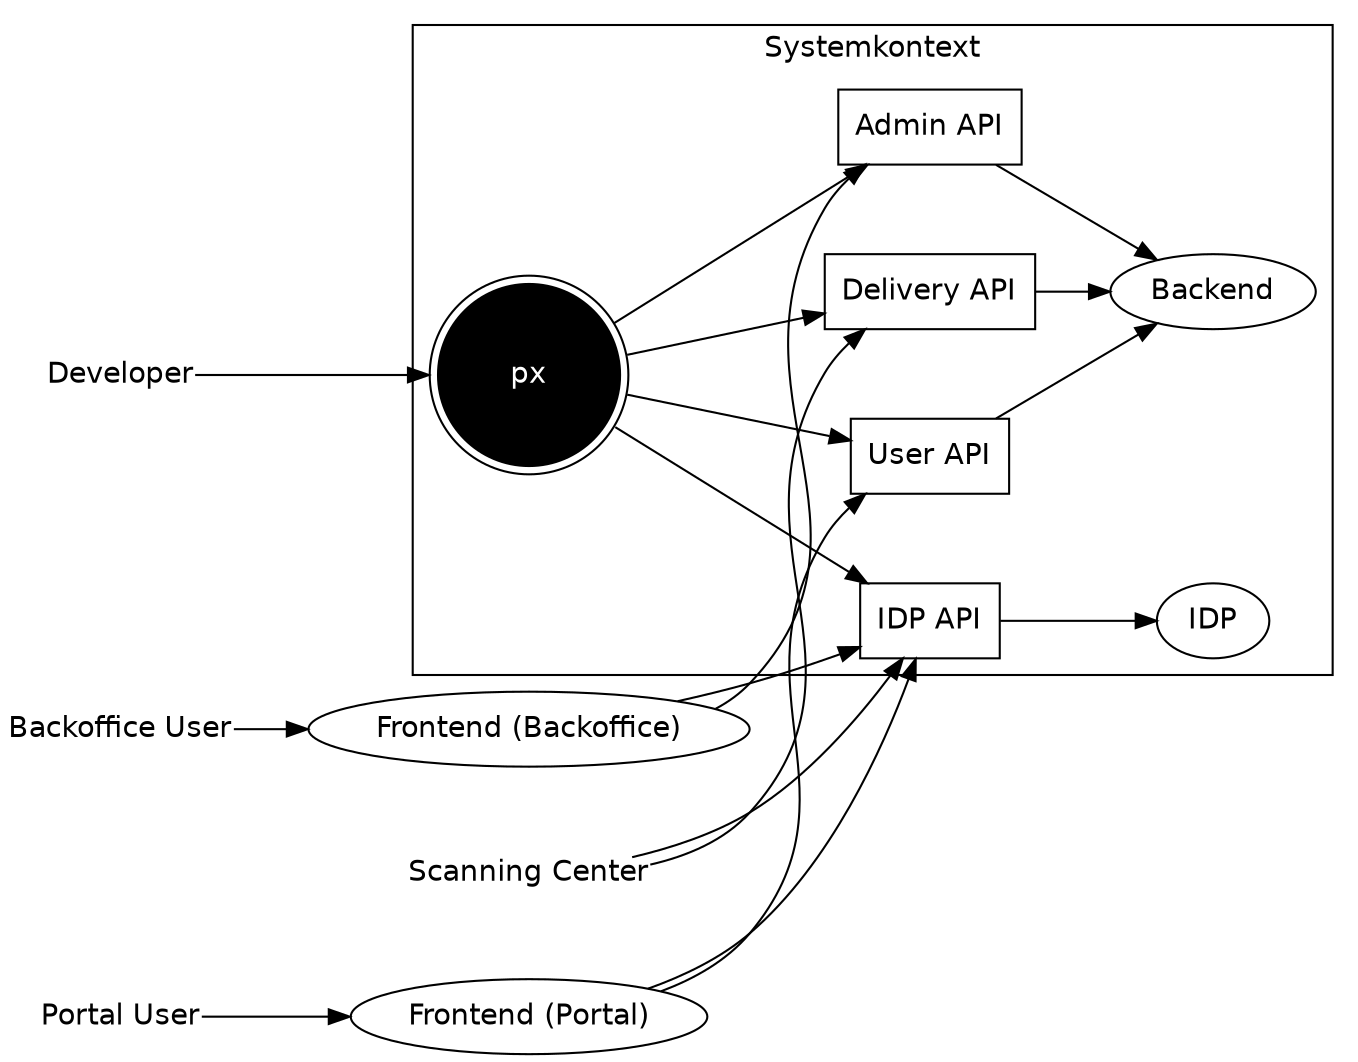
\includegraphics[width=\linewidth]{pics/kontextdiagramm.png}
	\caption{Kontextdiagramm: \texttt{px} als der Gegenstand der Arbeit innerhalb des Systemkontexts}
	\label{fig:kontextdiagramm}
\end{figure}

Im Kontextdiagramm (\imgref{fig:kontextdiagramm}) wird die zu entwickelnde Komponente \texttt{px} im Systemkontext von PEAX dargestellt. Andere Komponenten sind als Ellipsen, Schnittstellen als Rechtecke dargestellt. Ausserhalb vom Systemkontexts befindet sich die irrelevante Umgebung (d.h. die Frontend-Anwendungen). Die im Kontextdiagramm verwendeten Begriffe haben folgende Bedeutungen:

\begin{itemize}
	\item \texttt{px}: Der PEAX Command Line Client (Gegenstand der vorliegenden Arbeit)
	\item Developer: Ein Softwareentwickler (im weitesten Sinne) bei PEAX, der \texttt{px} verwendet.
	\item Backoffice User: Ein PEAX-Angestellter mit administrativen Befugnissen (Benutzerverwaltung).
	\item Portal User: Ein Benutzer des PEAX-Portals (Kunde).
	\item Scanning Center: Zulieferfirma, welche die umgeleitete Papierpost der PEAX-Kunden erhält, diese einscannt und dem betreffenden Kunden ins Portal stellt.
	\item Frontend (Backoffice): Ein Web-GUI für administrative Tätigkeiten zum internen Gebrauch.
	\item Frontend (Portal): Ein Web-GUI für die Kunden von PEAX (das eigentliche Portal).
	\item Admin API: RESTful API für administrative Aufgaben
	\item Agent API: RESTful API zum Einliefern von Dokumenten über Zulieferer
	\item User API: RESTful API für die Operationen der Kunden
	\item IDP API: RESTful API für das Token-Management (OAuth 2.0/OpenID Connect)
	\item Backend: Serverseitige Software mit Businesslogik und Datenspeicher
	\item IDP: Identity Provider, API-übergreifende Benutzer- und Zugangsverwaltung (AuthN/AuthZ)
\end{itemize}

\subsubsection{Architektur und Designentscheide}

Die Architektur der Anwendung ist im \secref{sec:Realisierung}, Designentscheide sind im \secref{sec:Ideen-und-Konzepte} beschrieben.

Limitierende Mengengerüste sind im relevanten Systemkontext aufseiten des Backends zu verorten und liegen daher nicht im Scope der vorliegenden Arbeit. Lokal fallen pro Umgebung maximal zwei Token Pairs (Access und Refresh Token; User- und Agent-API) an, d.h. vier Tokens. Mit den bis dato acht verfügbaren Umgebungen ergibt dies eine maximale Anzahl von 32 gleichzeitig abzuspeichernden Tokens. Ein Access Token, der grössere der beiden Tokens, hat eine Länge von ca. 1800 Bytes; der kürzere Refresh Token wiegt die zusätzlichen abgespeicherten Informationen (PEAX ID, Token Type usw.) und den JSON-Overhead bei weitem auf, sodass lokal maximal 57'600 Bytes abzuspeichern sind. Die ausführbaren \texttt{px}-Dateien sind mit ca. 7.5 bis 9.5 MB (je nach Plattform) wesentlich grösser. 

\subsubsection{Schnittstellen}

Als externe Schnittstellen verwendet \texttt{px} die im Kontextdiagramm (\imgref{fig:kontextdiagramm}) verwendeten APIs des Backends und des IDPs. Diese Interaktionen sind im Kapitel \secref{sec:Realisierung} beschrieben. Weiter interagiert \texttt{px} mit dem Dateisystem (Token Store \texttt{\~{}/.px-tokens}, temporäre Dateien für Payloads) des Betriebssystems. Die Schnittstelle zum nativen Keystore wurde mit der Fremdkomponente \texttt{go-keyring} von \textsc{Zalando} (\secref{sec:Go-Keyring}) gelöst.

Die internen Schnittstellen sind am besten in der Package-Übersicht (\secref{sec:Architektur-Package-Übersicht}) ersichtlich.\footnote{Führt man im Quellcodeverzeichnis von \texttt{px} den Befehl \texttt{godoc} aus, kann die Quellcodedokumentation komfortabel im Browser unter \url{http://localhost:6060/pkg/px/} betrachtet werden.}

Die Benutzerschnittstelle ist im Kapitel \secref{sec:Swiss-Army-Knive} konzeptionell und anhand konkreter Beispiele erläutert. 

\subsubsection{Environment-Anforderungen}

An die Umgebung stellt \texttt{px} nur geringe Anforderungen. Zur Ausführung wird \textsc{macOS}, \textsc{Windows} oder \textsc{Linux} in einer mehr oder weniger aktuellen Version benötigt. Tests wurden auf \textsc{macOS Catalina}, \textsc{Windows 10} und \textsc{Arch Linux} erfolgreich ausgeführt. Zur Bedienung wird eine \textsc{Unix}-Shell wie z.B. \textsc{Bash} empfohlen, wobei \texttt{px} auch mit \texttt{cmd.exe} oder der \textsc{PowerShell} funktioniert. Eine funktionierende Internetverbindung wird angenommen.

Grundsätzlich kann \texttt{px} auf allen Betriebssystemen und Plattformen kompiliert werden, auf denen \textsc{Go} läuft.\footnote{siehe \url{https://github.com/golang/go/wiki/MinimumRequirements}} Die aktuelle Build-Konfiguration geht von der \texttt{amd64}-Architek\-tur aus. Mithilfe der Umgebungsvariablen \texttt{GOOS} und \texttt{GOARCH} kann \texttt{px} auf eine Vielzahl von Umgebungen cross-kompiliert werden.\footnote{\url{https://gist.github.com/asukakenji/f15ba7e588ac42795f421b48b8aede63} bietet eine gute Übersicht.}

Dateien werden jeweils mit dem Encoding \texttt{UTF-8} gelesen und geschrieben. Für Quellcodedateien ist dies bei \textsc{Go} sogar eine verbindliche Vorgabe.\footnote{siehe \url{https://golang.org/ref/spec\#Source_code_representation}}

\subsection{Technologie-Evaluation}

Im Bereich der Technologie gilt es vor allem eine passende Programmiersprache auszuwählen. Die API von PEAX wird bereits durch den Projektrahmen vorgegeben, und dadurch auch die Protokolle OAuth 2.0 und HTTP.

\subsubsection{Programmiersprache}

Aus der Aufgabenstellung und dem Umfeld bei PEAX ergeben sich folgende nicht-funktio\-nale Anforderungen an die zu erstellende Software:

\begin{description}
    \item[Installation] Die Software soll sich einfach installieren lassen.
    \item[Umgebung] Es dürfen keine besonderen Anforderungen an die Umgebung gestellt werden, auf der \texttt{px} läuft.
    \item[Plattformen] Die Software soll auf allen gängigen, d.h. bei PEAX eingesetzten, Betriebssystemen (\textsc{Windows}, \textsc{macOS}, \textsc{Linux}) lauffähig sein.
    \item[Einheitlichkeit] Der Client soll überall die gleiche Befehlssyntax haben.
    \item[Performance] Ein Command Line Client soll in Skripten verwendet werden können, wodurch das Programm sehr oft in kurzem Zeitraum aufgestartet werden muss.
\end{description}

\textsc{Java}, das bei PEAX im Backend-Bereich zum Einsatz kommt, erfordert die lokale Installation einer JRE in der richtigen Version, was bei Frontend-Entwicklern nicht gegeben ist. Ausserdem werden Wrapper-Skripts benötigt (\texttt{java -jar px.jar} ist nicht praktikabel).

\textsc{Python}, \textsc{Ruby}, \textsc{Perl} und andere Skriptsprachen benötigen ebenfalls einen vorinstallierten Interpreter in der richtigen Version.

Zwar gibt es mit Mono eine Variante von .Net, die überall lauffähig ist, hier werden aber wiederum eine Laufzeitumgebung bzw. vorinstallierte Libraries benötigt.

Für die Problemstellung am besten geeignet sind kompilierte Sprachen (C, C++, \textsc{Go}, \textsc{Rust}, \textsc{Nim}). Mit einer statischen Kompilierung lässt sich das ganze Programm in eine einzige Binärdatei überführen, welches denkbar einfach zu installieren ist (Kopieren nach einem der Verzeichnisse innerhalb von \texttt{\$PATH}).

Für \textsc{JavaScript}, das bei PEAX im Frontend zum Einsatz kommt, gibt es mit \textsc{QuickJS}\footnote{\url{https://bellard.org/quickjs/}} seit kurzem die Möglichkeit, \textsc{JavaScript} zu Binärdateien zu kompilieren. Dies funktioniert aber nicht auf allen Plattformen, ausserdem ist \textsc{QuickJS} noch experminentell und noch nicht für den produktiven Einsatz geeignet.

Um ein Projekt vom gegebenen Umfang innerhalb eines Semesters umsetzen zu können, sind Vorkenntnisse in der einzusetzenden Programmiersprache zwar nicht zwingend, können das Risiko des Scheiterns aber erheblich senken. Gerade bei der Abschätzung von Aufwänden ist Vertrautheit mit den einzusetzenden Werkzeugen sehr hilfreich.

Was (statisch) kompilierte Programmiersprachen betrifft, konnte der Autor dieser Arbeit bereits Erfahrungen mit C, \textsc{Go} und \textsc{Rust} sammeln. Das manuelle Speichermanagement in C (u.a. auch bei Strings) ist einerseits ein grosses Risiko (Buffer Overflows, Segmentation Faults), und wirkt sich andererseits negativ auf das Entwicklungstempo aus. In die engere Auswahl kommen somit \textsc{Go} und \textsc{Rust}.

Im Folgenden werden die gemachten Erfahrungen und die dabei empfundenen Vor- und Nachteile mit den Programmiersprachen \textsc{Go} und \textsc{Rust} einander gegenübergestellt.

\subsubsection{\textsc{Go}}

Mit \textsc{Go} konnte der Autor dieser Arbeit bereits einges an Erfahrung sammeln. So wurde neben dem Prototyp zu \texttt{px} bereits die Testat-Aufgabe im Modul Software Testing\footnote{\url{https://github.com/patrickbucher/getting-to-philosophy}}, ein Thumbnailer\footnote{\url{https://github.com/patrickbucher/thumbnailer}} sowie zahlreiche Utilities\footnote{\url{https://github.com/patrickbucher/go-scratch}} (viele darunter als HTTP-Clients) in \textsc{Go} entwickelt. Dabei wurden folgende Vor- und Nachteile ermittelt:

\begin{itemize}
    \item[+] aufgrund weniger Keywords und Features einfach zu lernen
    \item[+] hervorragendes Tooling out-of-the-box
    \item[+] Cross-Compilation ohne Zusatztools auf alle unterstützte Plattformen möglich
    \item[+] schnelle Kompilierung
    \item[+] umfassende Standard-Library, die u.a. ein hervorrangendes HTTP-Package beinhaltet
    \item[+] persönlich bereits viel (positive) Erfahrungen damit gesammelt
    \item[+] wird bereits für andere bei PEAX gebräuchliche CLI-Tools eingesetzt (\texttt{oc}, \texttt{docker})
    \item[+] fügt sich sehr gut in die \textsc{Unix}-Philosophie ein (Tooling, Libraries)
    \item[+] Einfaches Interface für nebenläufige Programmierung (Goroutines und Channels)
    \item[+] geringer Memory-Verbrach bei relativ hoher Performance\footnote{\url{https://benchmarksgame-team.pages.debian.net/benchmarksgame/fastest/go.html}}
    \item[-] keine Features wie Generics, Exceptions und \texttt{filter}/\texttt{map}/\texttt{reduce}
    \item[-] Binaries fallen relativ gross aus\footnote{\url{https://golang.org/doc/faq\#Why\_is\_my\_trivial\_program\_such\_a\_large\_binary}}
    \item[-] Error-Handling aufwändig und teils repetitiv
\end{itemize}

\subsubsection{\textsc{Rust}}

Der Autor dieser Arbeit konnte sich bereits letztes Jahr im Rahmen des Moduls \textit{Programming Concepts and Paradigms} an der HSLU Informatik mit \textsc{Rust} befassen \cite[S. 12]{pcp-rust}. Nach selbständiger Beschäftigung mit dieser Programmiersprache im Sommer können (teils ergänzend) folgende Vor- und Nachteile genannt werden:

\begin{itemize}
    \item[+] viele moderne Features (Generics, \texttt{filter}/\texttt{map}/\texttt{reduce})
    \item[+] hervorragendes Typsystem
    \item[+] gutes und ausgereiftes Tooling
    \item[+] weder manuelles Memory-Management noch Garbage Collector nötig
    \item[+] Pattern Matching führt zu sehr solidem Code
    \item[+] gegenüber \textsc{Go} schlankere Binaries
    \item[+] kommt bereits in der Form einiger CLI-Tools persönlich zum Einsatz (\texttt{rg}, \texttt{bat}, \texttt{hexyl}, \texttt{battop})
    \item[+] erstklassige Performance (im Bereich von C/C++) bei geringem Speicherverbrauch\footnote{\url{https://benchmarksgame-team.pages.debian.net/benchmarksgame/fastest/rust-go.html}}
    \item[-] hohe Einstiegshürde und lange Einarbeitungszeit
    \item[-] Cross-Compilation benötigt Zusatztools
    \item[-] noch keine praxisnahe Erfahrung damit gesammelt
    \item[-] aufgrund schlanker Standard Library auf viele Dependencies angewiesen
\end{itemize}

\subsubsection{Entscheidung Programmiersprache}
\label{sec:Entscheidung-Programmiersprache}

\textsc{Rust} hat gegenüber \textsc{Go} einige unbestreitbare Vorzüge (Memory Management, Typsystem, Ausdrucksstärke, Eliminierung ganzer Fehlerklassen, Performance, schlankere Binärdateien). Bezogen auf das umzusetzende Projekt haben jedoch einige davon kaum einen wichtigen Stellenwert (etwa Performance und Zero-Cost Abstractions). Hier fallen die Vorzüge von \textsc{Go} (umfassende Standard Library, Cross-Compilation) wesentlich stärker ins Gewicht.

Gerade die absichtlich schlank gehaltene Standard Library von \textsc{Rust}, die etwa zur Generierung von Zufallszahlen bereits externe Abhängigkeiten erfordert\footnote{\url{https://doc.rust-lang.org/book/ch02-00-guessing-game-tutorial.html\#using-a-crate-to-get-more-functionality}}, dürfte sich im vorliegenden Projektrahmen negativ auswirken, zumal die Evaluation verschiedener Libraries einen sehr hohen Zusatzaufwand erfordert.

Da \textsc{Go} bereits bei der Entwicklung des Prototypen von \texttt{px} erfolgreich zum Einsatz kam, und einige Projektaspekte (grundlegende CI-Pipeline, \texttt{Makefile} für Cross-Compilation und Packaging) bereits damit implementiert werden konnten, soll \textsc{Go} für das vorliegende Projekt den Vorzug erhalten.

Eine spätere Neuimplementierung von \texttt{px} in \textsc{Rust} wäre ein technisch durchaus interessantes, wenn auch praktisch wenig dringendes ‒ als Fallstudie aber durchaus lohnendes ‒ Unterfangen.

\subsection{Libraries}

Wie bereits in \secref{sec:Go-Keyring} geschildert, wird nur eine einzige Fremdkomponente verwendet: Das Package \texttt{go-keyring} von \textsc{Zalando}. Für die sichere Passworteingabe wird ein SSH-Terminal (\texttt{golang.org/x/crypto}) verwendet, das zu den halboffiziellen \textsc{Go}-Packages gehört.\footnote{Die \textsc{Go}-Packages unter \texttt{golang.org/x} sind vergleichbar mit den \textsc{Java}-Libraries unter \texttt{javax}.}

\subsection{Weitere Dokumente}
\label{apx:WeitereDokumente}

\begin{description}
    \item[Projektauftrag] Im Projektauftrag (\texttt{Anhang/Projektauftrag.pdf}) ist die Aufgabe beschrieben, wie sie zu Beginn des Projekts definiert worden ist.
    \item[Projektplan] Der Projektplan (\texttt{Anhang/Projektplan.pdf}) besteht aus einem Rahmenplan, einem Meilensteinplan und einem Wochenplan.
    \item[Backlog] Das Backlog (\texttt{Anhang/Backlog.pdf}) enthält die einzelnen User Stories, die Sprint-Planung, Umsetzungsnotizen zu einzelnen User Stories mit Testprotokolle dazu, sowie Informationen zu manuellen Tests und gefundenen Bugs.
    \item[Meilensteinbericht 1] Der erste Meilensteinbericht (\texttt{Anhang/Meilensteinbericht-1.pdf}) beschreibt die Vorgeschichte des Projekts und die Phase der Projektinitialisierung.
    \item[Meilensteinbericht 2] In diesem Meilensteinbericht (\texttt{Anhang/Meilensteinbericht-2.pdf}) geht es um die ersten beiden Sprints.
    \item[Meilensteinbericht 3] In diesem Meilensteinbericht (\texttt{Anhang/Meilensteinbericht-3.pdf}) geht es um die letzten beiden Sprints.
    \item[Arbeitsjournal] Im Arbeitsjournal (\texttt{Anhang/Arbeitsjournal.pdf}) sind die einzelnen Aufwände auf halbe Stunden gerundet nach Bereich ‒ Projekt(administration), Dokumentation, Umsetzung ‒ rapportiert. Mithilfe eines AWK-Skripts können die Aufwände nach Bereich und User Story ausgewertet werden.
\end{description}

\newpage

%\section{Einstiegsbeispiel}

\begin{lstlisting}[language=Go,caption={Some Go Code}]
package main

import (
	"fmt"
	"log"
	"os"

	"gopl.io/ch05/links"
)

// breadthFirst calls f for each item in the worklist.
// Any items returned by f are added to the worklist.
// f is called at most once for each item.
func breadthFirst(f func(item string) []string, worklist []string) {
	seen := make(map[string]bool)
	for len(worklist) > 0 {
		items := worklist
		worklist = nil
		for _, item := range items {
			if !seen[item] {
				seen[item] = true
				worklist = append(worklist, f(item)...)
			}
		}
	}
}

func crawl(url string) []string {
	fmt.Println(url)
	list, err := links.Extract(url)
	if err != nil {
		log.Print(err)
	}
	return list
}

func main() {
	// Crawl the web breadth-first,
	// starting from the command-line arguments.
	breadthFirst(crawl, os.Args[1:])
}
\end{lstlisting}

%\newpage

\bibliographystyle{apacite}
\bibliography{document}
\newpage

\listoffigures
\addcontentsline{toc}{section}{Abbildungsverzeichnis}
\newpage

\listoftables
\addcontentsline{toc}{section}{Tabellenverzeichnis}
\newpage

\lstlistoflistings
\addcontentsline{toc}{section}{Verzeichnis der Codebeispiele}

\end{document}
